\subsection{IFIT1, IFIT3, and IFIT5 Localisation with Regards to RSV Pseudo-IBs} \label{subsec:IFIT1, IFIT3, and IFIT5 Localisation with Regards to RSV Pseudo-IBs}
The cells, irrespective of the chosen cell line, were maintained and passaged under standard conditions, as outlined in Sections \ref{sec:Cell Culture} and \ref{subsec:Passaging and Seeding Cells}. Transfections involved the use of human or bovine RSV \textit{N} or \textit{P} codon-optimised ORFs, housed within pcDNA3.1 plasmid backbones, employing TransIT-X2 at a 1:2 ratio, as detailed in Section \ref{subsec:Transfecting Cells}. Despite attempts with lipofectamine 3000, which, although similar in transfection efficiencies, exhibited increased cellular toxicity (data not presented), we consistently utilized TransIT-X2 for transfection. The conditions included transfecting 500 $\mu$g of each plasmid per 50,000 cells seeded in a 24-well plate per well, following optimisation of various parameters such as total DNA used, seeding density, and plasmid ratios (data not presented).

Initial experiments were conducted in human embryonic kidney (HEK) 293T cells, characterised by high plasmid transfection permissivity, often achieving efficiencies exceeding 90\%. However, these cells presented challenges for confocal microscopy and subsequent image analysis due to their small nucleus-to-cytoplasm ratio and adherence difficulties during treatment or washes. Despite these challenges, the initial staining experiments for IFIT1 and IFIT2 (Section \ref{subsec:Dissecting the Differential IFIT2 Antibody Staining}) were conducted using HEK293T cells. Subsequently, a transition to alternative cell lines was deemed necessary. HeLa and Vero cell lines were evaluated based on their transfection efficiency, cell morphology, and culture simplicity. HeLa, derived from human uterine epithelial cancer cells, was considered more suitable for our purposes. In contrast, the Vero cell line originates from the kidney epithelial tissue of adult African green monkeys (\textit{Cercopithecus Aethiops}) \cite{Simizu1967CharacterizationVero}. Initial optimisation experiments revealed minimal transfection efficiency in the HeLa cell line under all tested conditions (data not shown). On the other hand, Vero cells consistently exhibited transfection, albeit with lower efficiencies compared to those observed in the HEK293T cell line, approximately 30\% and 90\% respectively (data not shown). Nevertheless, this level of transfection was deemed sufficient for subsequent confocal microscopy experiments.

Vero cells are commonly employed for propagating and studying various viruses, particularly bovine RSV. While the optimal scenario would involve detecting endogenous human IFITs interacting with RSV pseudo-inclusion bodies, it is crucial to note that primate IFITs, including those of monkeys, are phylogenetically more akin to human IFITs than bovine IFITs \cite{Zhou2013InterferonDefense.}. As demonstrated in the previous chapter, the interactions of human and bovine IFITs exhibit considerable consistency. Therefore, exploring the colocalisation of monkey IFITs with human or bovine pIBs holds promise for gaining valuable insights into these interactions.

\begin{figure}
    \begin{subfigure}{0.495\textwidth}
        \caption{}
        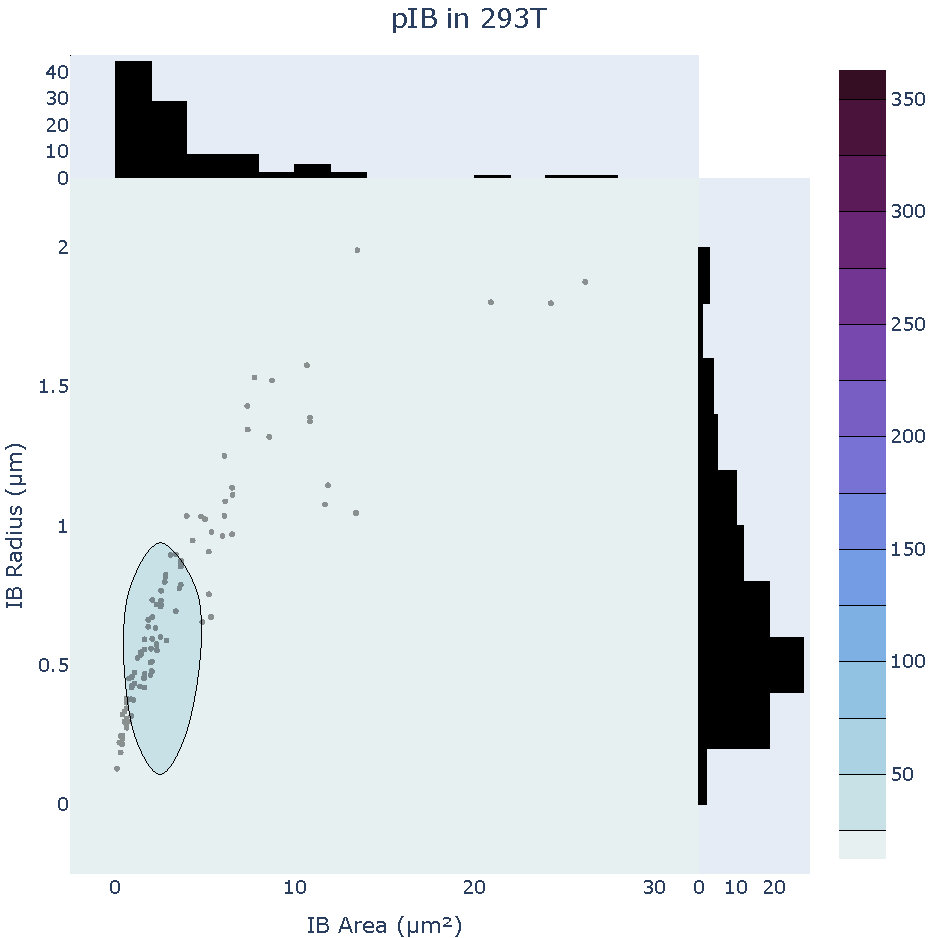
\includegraphics[width=\textwidth]{09. Chapter 4/Figs/01. pIB/01. pIB characterisation/01. heatmap_pib-293t.pdf} 
    \end{subfigure}
    \hfill
    \begin{subfigure}{0.495\textwidth}
        \caption{}
        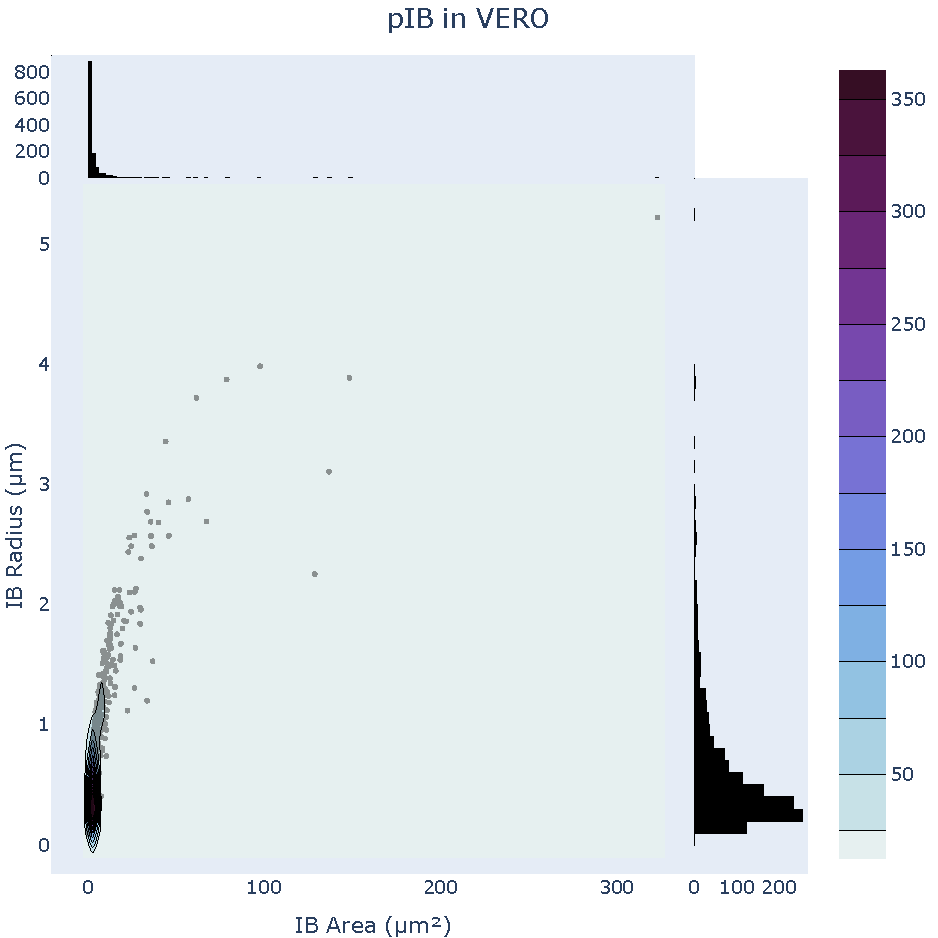
\includegraphics[width=\textwidth]{09. Chapter 4/Figs/01. pIB/01. pIB characterisation/02. heatmap_pib-vero.pdf}
    \end{subfigure}
    \caption[Size Characterisation of Pseudo Inclusion Bodies Across Different Cell Lines.]{\textbf{Size Characterisation of Pseudo Inclusion Bodies Across Different Cell Lines.} This figure presents the relationship between the measured area (\(\mu \mbox{m}^2\)) and diameter (\(\mu \mbox{m}\)) of individual pseudo inclusion bodies (pIBs) as observed within the scope of this study. Additionally, the figure includes distinct population distributions depicted alongside the plots, representing (a) 103 observations from the 293T cell line and (b) 1321 observations from the Vero cell line. Contour plots are incorporated to elucidate the underlying density of individual IBs within the plots.}
    \label{fig:Size Characterisation of Pseudo Inclusion Bodies Across Different Cell Lines}
\end{figure}

We conducted a systematic observation and annotation of a total of 1424 pseudo-inclusion bodies, comprising 103 observations in the HEK293T cell line and 1321 observations in the Vero cell line. The relationship between their measured area and radius is illustrated in Figure \ref{fig:Size Characterisation of Pseudo Inclusion Bodies Across Different Cell Lines}. Pseudo-inclusion bodies in both cell lines generally conform to logarithmic curves, consistent with the expected relationship of the observed values. Notably, a substantial number of detected entities exhibit a larger measured area than the predicted radius, indicative of an elongated ellipsoidal shape. In the HEK293T cell line, the pseudo-inclusion bodies predominantly displayed a radius of 0.5 \(\mu \mbox{m}\), with the majority falling within the range of 0.25 \(\mu \mbox{m}\) to 1 \(\mu \mbox{m}\). Regarding the associated measured area, most pseudo-inclusion bodies ranged from 0.5 \(\mu \mbox{m}^2\) to 4 \(\mu \mbox{m}^2\). Contrastingly, in the Vero cell line, we observed a broader distribution of data, with pseudo-inclusion bodies measuring >5 \(\mu \mbox{m}\) in radius and >300 \(\mu \mbox{m}^2\) in area. Nevertheless, the majority of the detected entities in this cell line exhibited radii between 0.1 \(\mu \mbox{m}\) and 0.7 \(\mu \mbox{m}\), coupled with measured 2D areas ranging from 0.1 \(\mu \mbox{m}^2\) to 4 \(\mu \mbox{m}^2\).

\begin{figure}
    \centering
    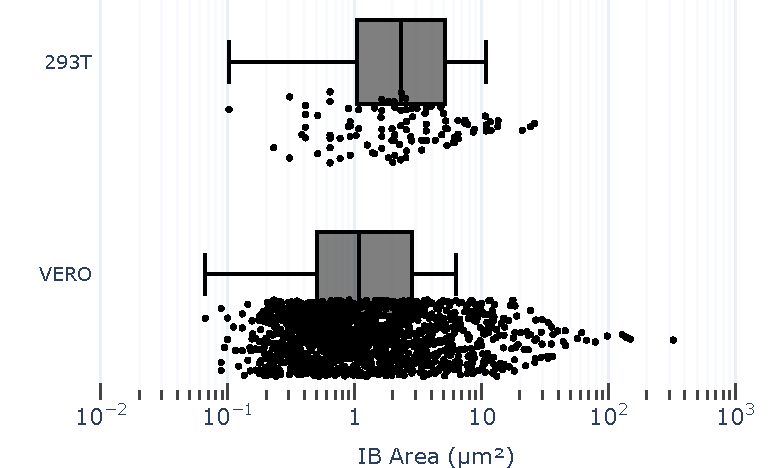
\includegraphics[width=0.75\linewidth]{09. Chapter 4/Figs/01. pIB/01. pIB characterisation/03. box-pib.pdf}
    \caption[The Distributions of pIB Areas Observed Per Cell Line.]{\textbf{The Distributions of pIB Areas Observed Per Cell Line.} The distribution of RSV pseudo inclusion body areas (\(\mu \mbox{m}^2\)), detected in this study are shown. A total of 103 observations were made in the 293T cell line, and 1321 observations in the Vero cell line.}
    \label{fig:The Distributions of pIB Areas Observed Per Cell Line}
\end{figure}

A more detailed view focusing solely on the distribution of measured areas per cell line can be observed in Figure \ref{fig:The Distributions of pIB Areas Observed Per Cell Line}. Notably, pIBs detected in the Vero cell line exhibit a broader range in terms of minimal and maximal measured areas compared to those in the 293T cell line. However, the median value in the 293T cell line surpasses that of the Vero cell line. Specifically, in the 293T cell line, we observed pIB areas ranging from sub 0.2 \(\mu \mbox{m}^2\) to supra 20 \(\mu \mbox{m}^2\), with a median value of 2.2 \(\mu \mbox{m}^2\). Conversely, in the Vero cell line, the observed pIBs spanned from sub 0.07 \(\mu \mbox{m}^2\) to supra 300 \(\mu \mbox{m}^2\), with a median value of 1 \(\mu \mbox{m}^2\). It is noteworthy that both median values are notably smaller than those observed in cell lines during infection (refer to Section \ref{subsec:IFIT Subcellular Localisation During Interferon Induction and RSV Infection}, Figure \ref{fig:The Distributions of IB Areas Observed Per Cell Line}). This finding aligns with literature reports, indicating that pIBs observed 24 hours post-transfection are considerably smaller than conventional inclusion bodies observed in infected cells after an equivalent passage of time \cite{Jobe2021BovineResponses}.

\begin{figure}
    \begin{subfigure}{0.495\textwidth}
        \caption{}
        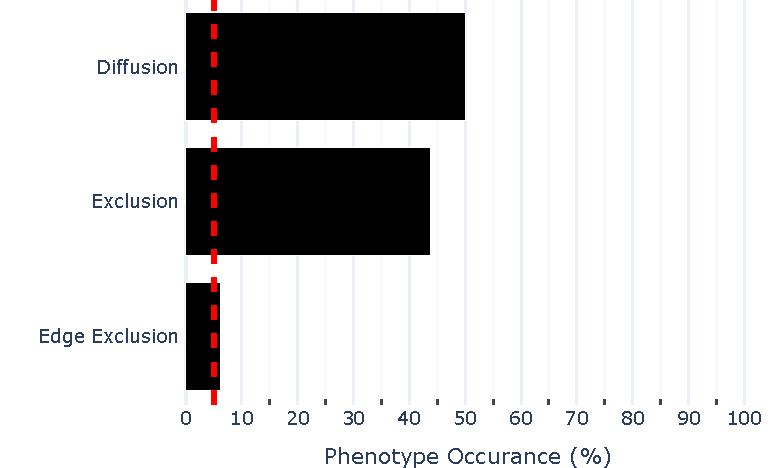
\includegraphics[width=1\linewidth]{09. Chapter 4/Figs/01. pIB/02. IFIT1/01. bar_i1_293t.pdf} 
    \end{subfigure}
    \begin{subfigure}{0.495\textwidth}
        \caption{}
        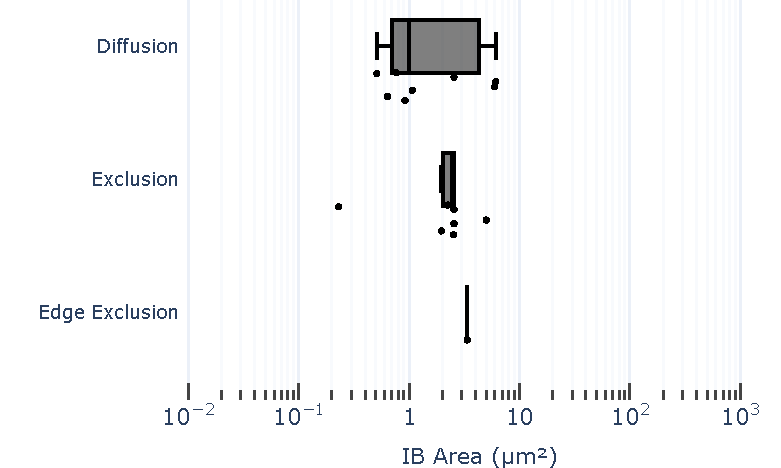
\includegraphics[width=1\linewidth]{09. Chapter 4/Figs/01. pIB/02. IFIT1/02. box_i1_293t.pdf}
    \end{subfigure}
    \caption[Phenotypic Interactions of Human IFIT1 with Human pIBs in the 293T Cell Line.]{\textbf{Phenotypic Interactions of Human IFIT1 with Human pIBs in the 293T Cell Line.} 293T cells were transfected with hRSV N and P containing plasmids using TransIT-X2 and were fixed after 24 hours. Cells were labelled with anti-RSV N and anti-IFIT1 antibodies and imaged on a confocal microscope. Panel (a) shows the percentual proportions of observed phenotypes between hRSV pseudo inclusion bodies and human IFIT1 (16 observations), with the red dotted line denoting the 5\% threshold, marking phenotypes considered relevant above this limit. Panel (b) shows the IB area in \(\mu \mbox{m}^2\) per observed relevant phenotype.}
    \label{fig:Phenotypic Interactions of Human IFIT1 with Human pIBs in the 293T Cell Line}
\end{figure}

\begin{figure}
    \centering
    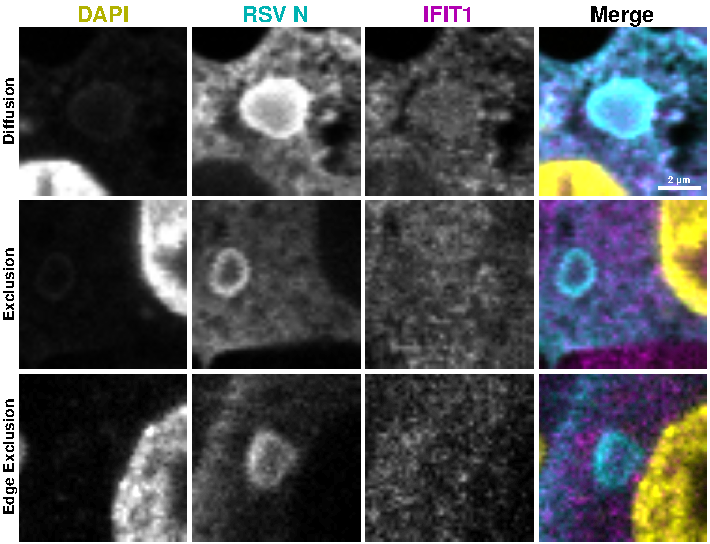
\includegraphics[width=1\linewidth]{09. Chapter 4/Figs/01. pIB/02. IFIT1/03. i1-293t-hnhp.pdf}
    \caption[Representative Images of Phenotypic Interactions of Human IFIT1 with Human pIBs in the 293T Cell Line.]{\textbf{Representative Images of Phenotypic Interactions of Human IFIT1 with Human pIBs in the 293T Cell Line.} 293T cells were transfected with hRSV N and P containing plasmids using TransIT-X2 and were fixed after 24 hours. Cellular nuclei were stained with DAPI (yellow), and cells were double-labelled with anti-RSV N (cyan) and anti-IFIT1 (magenta) antibodies. This figure showcases representative examples of relevant phenotypes in the interaction between human IFIT1 and hRSV pseudo-inclusion bodies. These phenotypes are presented in descending order based on their percentage proportions. The scale bar indicates 2 \(\mu \mbox{m}\).}
    \label{fig:Representative Images of Phenotypic Interactions of Human IFIT1 with Human pIBs in the 293T Cell Line}
\end{figure}

We obtained 16 observations of endogenous human IFIT1 and its interaction with hRSV pIBs in the 293T cell line. The observed phenotype frequencies, along with the measured pIB sizes, can be viewed in Figure \ref{fig:Phenotypic Interactions of Human IFIT1 with Human pIBs in the 293T Cell Line}, with representative images of these phenotypes shown in Figure \ref{fig:Representative Images of Phenotypic Interactions of Human IFIT1 with Human pIBs in the 293T Cell Line}. Half of the observations displayed the diffusion phenotype. This was predominantly observed in smaller pIBs with a typical size of 1 \(\mu \mbox{m}^2\) and ranging from 0.5 \(\mu \mbox{m}^2\) to 6 \(\mu \mbox{m}^2\) in size. The second most prevalent phenotype was exclusion, which occurred in 44\% of cases. The pIBs associated with this phenotype closely clustered at around 2.5 \(\mu \mbox{m}^2\), with two exceptions, i.e., one very small pIB (0.22 \(\mu \mbox{m}^2\)) and one relatively large pIB (5 \(\mu \mbox{m}^2\)). Lastly, we observed one pIB with a measured area of 3.3 \(\mu \mbox{m}^2\) which exhibited the exclusion phenotype. Overall, these data suggest that human IFIT1 does not associate with human RSV pIB structures, although this is based on a very limited set of observations.

\begin{figure}
    \begin{subfigure}{0.495\textwidth}
        \caption{}
        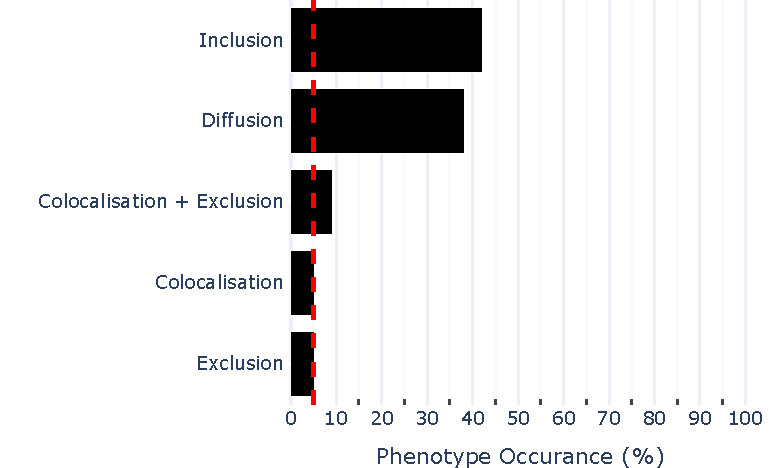
\includegraphics[width=1\linewidth]{09. Chapter 4/Figs/01. pIB/02. IFIT1/04. bar_i1_vero_hnhp.pdf} 
    \end{subfigure}
    \begin{subfigure}{0.495\textwidth}
        \caption{}
        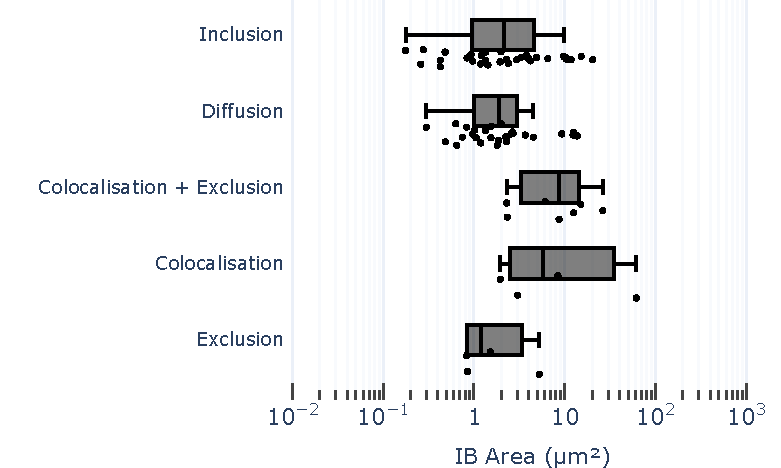
\includegraphics[width=1\linewidth]{09. Chapter 4/Figs/01. pIB/02. IFIT1/05. box_i1_vero_hnhp.pdf}
    \end{subfigure}
    \caption[Interaction Phenotypes of Monkey IFIT1 with Human pIBs in the Vero Cell Line.]{\textbf{Interaction Phenotypes of Monkey IFIT1 with Human pIBs in the Vero Cell Line.} Vero cells were transfected with hRSV N and P containing plasmids using TransIT-X2 and were fixed after 24 hours. Cells were labelled with anti-RSV N and anti-IFIT1 antibodies and imaged on a confocal microscope. Panel (a) shows the percentual proportions of observed phenotypes between hRSV pseudo inclusion bodies and monkey IFIT1 (76 observations), with the red dotted line denoting the 5\% threshold, marking phenotypes considered relevant above this limit. Panel (b) shows the IB area in \(\mu \mbox{m}^2\) per observed relevant phenotype.}
    \label{fig:Interaction Phenotypes of Monkey IFIT1 with Human pIBs in the VERO Cell Line}
\end{figure}

\begin{figure}
    \centering
    \includegraphics[width=1\linewidth]{09. Chapter 4/Figs/01. pIB/02. IFIT1/06. i1-vero-hnhp.pdf}
    \caption[Representative Images of Interaction Phenotypes of Monkey IFIT1 with Human pIBs in the Vero Cell Line.]{\textbf{Representative Images of Interaction Phenotypes of Monkey IFIT1 with Human pIBs in the Vero Cell Line.} Vero cells were transfected with hRSV N and P containing plasmids using TransIT-X2 and were fixed after 24 hours. Cellular nuclei were stained with DAPI (yellow), and cells were double-labelled with anti-RSV N (cyan) and anti-IFIT1 (magenta) antibodies. This figure showcases representative examples of relevant phenotypes in the interaction between monkey IFIT1 and hRSV pseudo-inclusion bodies. These phenotypes are presented in descending order based on their percentage proportions. The scale bar indicates 2 \(\mu \mbox{m}\).}
    \label{fig:Representative Images of Interaction Phenotypes of Monkey IFIT1 with Human pIBs in the VERO Cell Line}
\end{figure}

Next, we evaluated endogenous monkey IFIT1 interactions with pIBs created by transfection of hRSV \textit{N} and \textit{P} containing plasmids in the Vero cell line. The frequencies of occurrences of the interaction phenotypes based on 76 observations, along with the measured pIB areas per phenotype, are shown in Figure \ref{fig:Interaction Phenotypes of Monkey IFIT1 with Human pIBs in the VERO Cell Line}. Representative images of these phenotypes are shown in Figure \ref{fig:Representative Images of Interaction Phenotypes of Monkey IFIT1 with Human pIBs in the VERO Cell Line}. A notable 43\% of the observations depicted monkey IFIT1 forming intra-pIB inclusion, followed closely by a diffusion phenotype, observed in 38\% of instances. Further, 8\% of the observations revealed monkey IFIT1 colocalising with the edge of the pIB structure while being excluded from the primary pIB structure. Both colocalisation and exclusion phenotypes individually occurred in 5\% of cases each. Regarding the size profile of hRSV pIBs associated with these phenotypes, inclusion was observed across a diverse range of pIB sizes, spanning from sub 0.2 \(\mu \mbox{m}^2\) to supra 20 \(\mu \mbox{m}^2\), with a median size of 2 \(\mu \mbox{m}^2\). In contrast, the diffusion phenotype occurred in pIBs with a similar range of measured areas, displaying an identical median value of 2 \(\mu \mbox{m}^2\). Noteworthy distinctions emerged in the distribution of values between these two phenotypes. While the sizes of pIBs associated with the inclusion phenotype were evenly distributed across their minimal and maximal values, those linked with the diffusion phenotype clustered around 2 \(\mu \mbox{m}^2\). The colocalisation associated with the pIB exclusion phenotype occurred predominantly in larger pIBs, with a typical area of 9 \(\mu \mbox{m}^2\), absent in pIBs smaller than 2 \(\mu \mbox{m}^2\). Similarly, the colocalisation-phenotype associated hRSV pIBs exhibited larger sizes, with a median value of 6 \(\mu \mbox{m}^2\) and a minimal value of 2 \(\mu \mbox{m}^2\). Lastly, the exclusion phenotype occurred in 4 pIBs with a median 2D area of 1.1 \(\mu \mbox{m}^2\). In summary, within this simplified model, although the size of the pIB should not directly indicate a difference in the underlying pIB complexity, we observed a size-dependent association with phenotypes. Smaller, sub 1 \(\mu \mbox{m}^2\) pIBs predominantly exhibited inclusion and diffusion phenotypes, equally prevalent in these structures. In contrast, larger pIBs showcased inclusion, diffusion, and colocalisation associated with exclusion.

\begin{figure}
    \begin{subfigure}{0.495\textwidth}
        \caption{}
        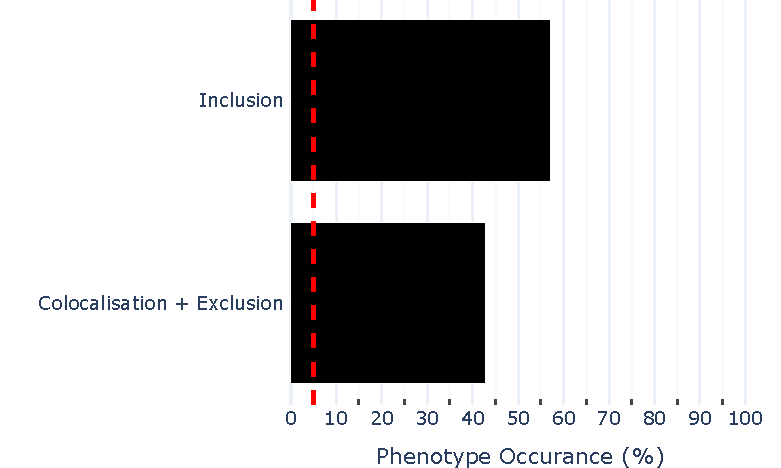
\includegraphics[width=1\linewidth]{09. Chapter 4/Figs/01. pIB/02. IFIT1/07. bar_i1_vero_bnbp.pdf}  
    \end{subfigure}
    \begin{subfigure}{0.495\textwidth}
        \caption{}
        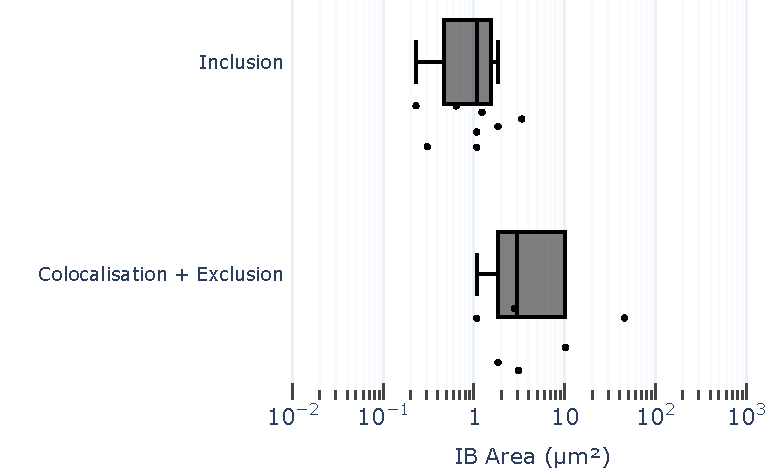
\includegraphics[width=1\linewidth]{09. Chapter 4/Figs/01. pIB/02. IFIT1/08. box_i1_vero_bnbp.pdf}
    \end{subfigure}
    \caption[Interaction Phenotypes of Monkey IFIT1 with Bovine pIBs in the Vero Cell Line.]{\textbf{Interaction Phenotypes of Monkey IFIT1 with Bovine pIBs in the Vero Cell Line.} Vero cells were transfected with bRSV N and P containing plasmids using TransIT-X2 and were fixed after 24 hours. Cells were labelled with anti-RSV N and anti-IFIT1 antibodies and imaged on a confocal microscope. Panel (a) shows the percentual proportions of observed phenotypes between bRSV pseudo inclusion bodies and monkey IFIT1 (14 observations), with the red dotted line denoting the 5\% threshold, marking phenotypes considered relevant above this limit. Panel (b) shows the IB area in \(\mu \mbox{m}^2\) per observed relevant phenotype.}
    \label{fig:Interaction Phenotypes of Monkey IFIT1 with Bovine pIBs in the VERO Cell Line}
\end{figure}

\begin{figure}
    \centering
    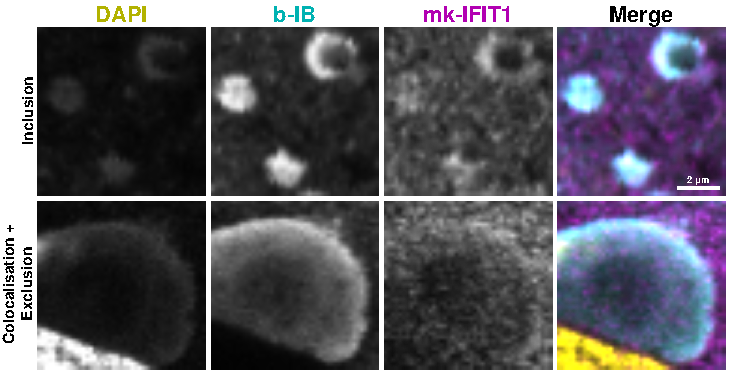
\includegraphics[width=1\linewidth]{09. Chapter 4/Figs/01. pIB/02. IFIT1/09. i1-vero-bnbp.pdf}
    \caption[Representative Images of Interaction Phenotypes of Monkey IFIT1 with Bovine pIBs in the Vero Cell Line.]{\textbf{Representative Images of Interaction Phenotypes of Monkey IFIT1 with Bovine pIBs in the Vero Cell Line.} Vero cells were transfected with bRSV N and P containing plasmids using TransIT-X2 and were fixed after 24 hours. Cellular nuclei were stained with DAPI (yellow), and cells were double-labelled with anti-RSV N (cyan) and anti-IFIT1 (magenta) antibodies. This figure showcases representative examples of relevant phenotypes in the interaction between monkey IFIT1 and bRSV pseudo-inclusion bodies. These phenotypes are presented in descending order based on their percentage proportions. The scale bar indicates 2 \(\mu \mbox{m}\).}
    \label{fig:Representative Images of Interaction Phenotypes of Monkey IFIT1 with Bovine pIBs in the VERO Cell Line}
\end{figure}

In the final exploration, we examined the interaction of monkey IFIT1, detected by the human IFIT1 antibody, with bovine RSV IBs through the transfection of bRSV \textit{N} and \textit{P} containing plasmids. Challenges arose due to consistently lower transfection efficiencies associated with these plasmids, resulting in a limited number of observations. Consequently, we encountered difficulties in generating sufficient samples to investigate endogenous monkey IFITs other than IFIT1 and IFIT2 using the A antibody, as detailed in Section \ref{subsec:Dissecting the Differential IFIT2 Antibody Staining}. Nonetheless, Figure \ref{fig:Interaction Phenotypes of Monkey IFIT1 with Bovine pIBs in the VERO Cell Line} presents the frequencies of occurrence of interaction phenotypes based on 14 observations, coupled with the measured pIB areas per phenotype. Representative images of these phenotypes are displayed in Figure \ref{fig:Representative Images of Interaction Phenotypes of Monkey IFIT1 with Bovine pIBs in the VERO Cell Line}. Remarkably, a pattern reminiscent of IFIT2 during RSV infection emerged, where only two phenotypes were observed: inclusion within the pIB structures, occurring at a frequency of 56\%, and colocalisation associated with pIB exclusion, occurring at a frequency of 44\%. The former predominated in smaller pIBs, with a median size of 1 \(\mu \mbox{m}^2\) and a maximum size of 4 \(\mu \mbox{m}^2\). In contrast, the colocalisation phenotype associated with exclusion manifested in pIBs with a typical size of 3 \(\mu \mbox{m}^2\). Despite an overlap in pIB sizes between the two phenotypes, sub 1 \(\mu \mbox{m}^2\) pIBs consistently correlated with inclusion, while supra 10 \(\mu \mbox{m}^2\) pIBs were consistently associated with colocalisation conjoined with exclusion.

Considering the entirety of the IFIT1-pIB interaction results, it suggests a differential propensity for pIB interaction between endogenous human and monkey IFIT1. Stating that, data obtained from the HEK293T cell line is limited in quantity and displays a size bias towards pIBs that are less than 6 \(\mu \mbox{m}^2\) in size. This observation does not align with the true diversity of pIB sizes observed in this study, as the aggregate of all pIBs observed in HEK293T cells indicates a sizeable population of supra 6 \(\mu \mbox{m}^2\) pIBs (Figure \ref{fig:The Distributions of pIB Areas Observed Per Cell Line}). In the Vero cell line transfected with hRSV \textit{N} and \textit{P} ORF-containing plasmids, we have observed phenotypes that imply direct interaction (colocalisation and colocalisation associated with exclusion) specifically in larger pIBs. This implies that the limited sample size and diversity of HEK293T observed hRSV pIBs are not sufficient to provide a true picture of IFIT1/pIB interaction. On the other hand, it can also be indicative of hIFIT1 not being recruited to the pIBs. Within the Vero cell line, we also observed differential results which depend on the species of the virus. While we have only observed direct interaction phenotypes of inclusion formation and pIB edge colocalisation with intra-pIB exclusion with the bRSV pIBs, we observed a more diverse interaction range in Vero cells with hRSV pIBs present in them. These phenotypes, however, all, with the exception of exclusion phenotype (which occurred only in 5\% of observations), imply IFIT1 having access to the pIB structure. It is intriguing to see the differences between human and bovine RSV pIB and their interaction with monkey IFIT1. This could suggest that the bovine pIB possibly lacks a mechanism that would prevent them from being targeted by the monkey IFIT1. Saying that, the bovine RSV pIB dataset lacks in-depth with regards to the number of observations, and thus the differences could also be attributed to the low frequency of diffusion or exclusion phenotypes. In that case, the results from Vero cell lines with either human or bovine RSV pIBs present would be almost identical.

\begin{figure}
    \begin{subfigure}{0.495\textwidth}
        \caption{}
        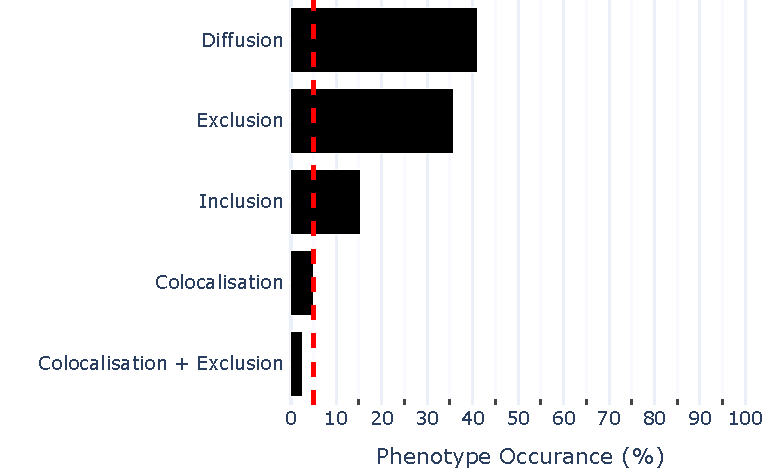
\includegraphics[width=1\linewidth]{09. Chapter 4/Figs/01. pIB/04. IFIT3/01. bar_i3_vero.pdf} 
    \end{subfigure}
    \begin{subfigure}{0.495\textwidth}
        \caption{}
        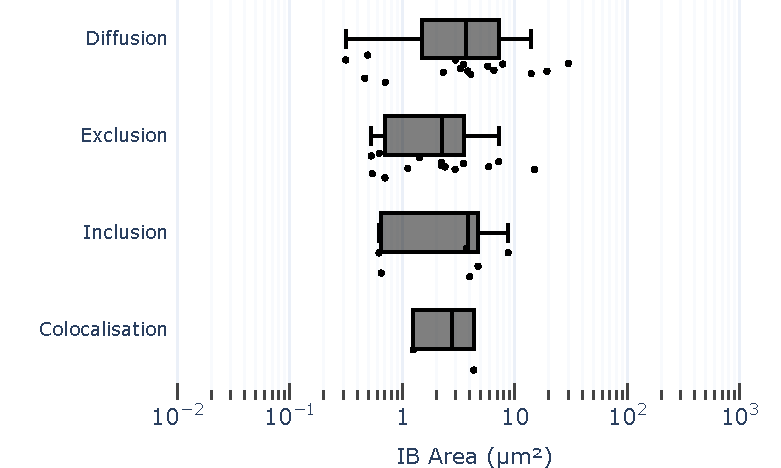
\includegraphics[width=1\linewidth]{09. Chapter 4/Figs/01. pIB/04. IFIT3/02. box_i3_vero.pdf}
    \end{subfigure}
    \caption[Interaction Phenotypes of Monkey IFIT3 with Human pIBs in the Vero Cell Line.]{\textbf{Interaction Phenotypes of Monkey IFIT3 with Human pIBs in the Vero Cell Line.} Vero cells were transfected with hRSV N and P containing plasmids using TransIT-X2 and were fixed after 24 hours. Cells were labelled with anti-RSV N and anti-IFIT3 antibodies and imaged on a confocal microscope. Panel (a) shows the percentual proportions of observed phenotypes between hRSV pseudo inclusion bodies and monkey IFIT3 (39 observations), with the red dotted line denoting the 5\% threshold, marking phenotypes considered relevant above this limit. Panel (b) shows the IB area in \(\mu \mbox{m}^2\) per observed relevant phenotype.}
    \label{fig:Interaction Phenotypes of Monkey IFIT3 with Human pIBs in the VERO Cell Line}
\end{figure}

\begin{figure}
    \centering
    \includegraphics[width=1\linewidth]{09. Chapter 4/Figs/01. pIB/04. IFIT3/03. i3-vero-hnhp.pdf}
    \caption[Representative Images of Interaction Phenotypes of Monkey IFIT3 with Human pIBs in the Vero Cell Line.]{\textbf{Representative Images of Interaction Phenotypes of Monkey IFIT3 with Human pIBs in the Vero Cell Line.} Vero cells were transfected with hRSV N and P containing plasmids using TransIT-X2 and were fixed after 24 hours. Cellular nuclei were stained with DAPI (yellow), and cells were double-labelled with anti-RSV N (cyan) and anti-IFIT3 (magenta) antibodies. This figure showcases representative examples of relevant phenotypes in the interaction between monkey IFIT3 and hRSV pseudo-inclusion bodies. These phenotypes are presented in descending order based on their percentage proportions. The scale bar indicates 2 \(\mu \mbox{m}\).}
    \label{fig:Representative Images of Interaction Phenotypes of Monkey IFIT3 with Human pIBs in the VERO Cell Line}
\end{figure}

Next, we explored the interaction of IFIT3 with RSV pseudo-inclusion bodies. Unfortunately, attempts to generate samples comprising both HEK293T cells transfected with hRSV \textit{N} and \textit{P}, and Vero cells transfected with bRSV \textit{N} and \textit{P} for staining with IFIT3 were unsuccessful. Consequently, we present the analysis of monkey IFIT3 interaction with hRSV pIBs. The frequencies of observed phenotypes within 39 observations, along with the measured pIB sizes per phenotype occurring with more than 5\% frequency, are depicted in Figure \ref{fig:Interaction Phenotypes of Monkey IFIT3 with Human pIBs in the VERO Cell Line}. Representative images of phenotypes occurring with at least 5\% frequency are shown in Figure \ref{fig:Representative Images of Interaction Phenotypes of Monkey IFIT3 with Human pIBs in the VERO Cell Line}. The most prevalent phenotype is diffusion throughout the pIB structure, occurring in 41\% of observations. This is closely followed by an exclusion phenotype, observed in 36\% of cases. Monkey IFIT3 forming intra-pIB inclusions were observed in 15\% of cases. Lastly, 5\% of observations showed a colocalisation phenotype, while 3\% displayed colocalisation associated with exclusion. Regarding the size profile of the IBs associated with different phenotypes occurring with at least 5\% frequency, their median values seem quite similar. However, they encompass a progressively narrower range of values as the occurrence frequency decreases. In more detail, the diffusion phenotype median pIB size was 4 \(\mu \mbox{m}^2\), ranging from 0.3 \(\mu \mbox{m}^2\) to 30 \(\mu \mbox{m}^2\). The exclusion phenotype-associated median area value was 2 \(\mu \mbox{m}^2\), with detected pIB sizes ranging from sub-0.6 \(\mu \mbox{m}^2\) to supra-10 \(\mu \mbox{m}^2\). The size values of inclusion-associated pIBs clustered at around 3 \(\mu \mbox{m}^2\), ranging from two observations at 6 \(\mu \mbox{m}^2\) to one observation at 9 \(\mu \mbox{m}^2\). Lastly, the pIBs associated with the colocalisation phenotype had sizes of 1.3 \(\mu \mbox{m}^2\) and 4.3 \(\mu \mbox{m}^2\). In most cases, monkey IFIT3 does not appear to directly interact with hRSV pIB structures. However, in a quarter of the cases, it either forms inclusions or associates with the edge of the pIB structure. This data aligns with our earlier investigation where IFIT3 predominantly exhibited exclusion and diffusion phenotypes during RSV infection.

\begin{figure}
    \begin{subfigure}{0.495\textwidth}
        \caption{}
        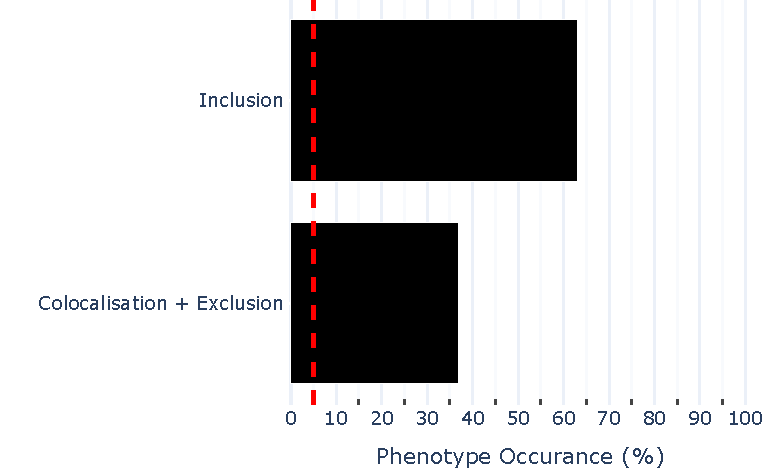
\includegraphics[width=1\linewidth]{09. Chapter 4/Figs/01. pIB/05. IFIT5/01. bar_i5_vero.pdf} 
    \end{subfigure}
    \begin{subfigure}{0.495\textwidth}
        \caption{}
        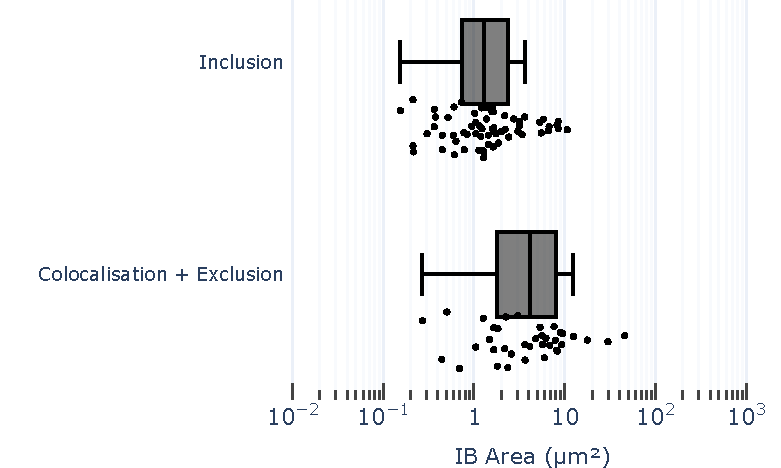
\includegraphics[width=1\linewidth]{09. Chapter 4/Figs/01. pIB/05. IFIT5/02. box_i5_vero.pdf}
    \end{subfigure}
    \caption[Interaction Phenotypes of Monkey IFIT5 with Human pIBs in the Vero Cell Line.]{\textbf{Interaction Phenotypes of Monkey IFIT5 with Human pIBs in the Vero Cell Line.} Vero cells were transfected with hRSV N and P containing plasmids using TransIT-X2 and were fixed after 24 hours. Cells were labelled with anti-RSV N and anti-IFIT5 antibodies and imaged on a confocal microscope. Panel (a) shows the percentual proportions of observed phenotypes between hRSV pseudo inclusion bodies and monkey IFIT5 (100 observations), with the red dotted line denoting the 5\% threshold, marking phenotypes considered relevant above this limit. Panel (b) shows the IB area in \(\mu \mbox{m}^2\) per observed relevant phenotype.}
    \label{fig:Interaction Phenotypes of Monkey IFIT5 with Human pIBs in the VERO Cell Line}
\end{figure}

\begin{figure}
    \centering
    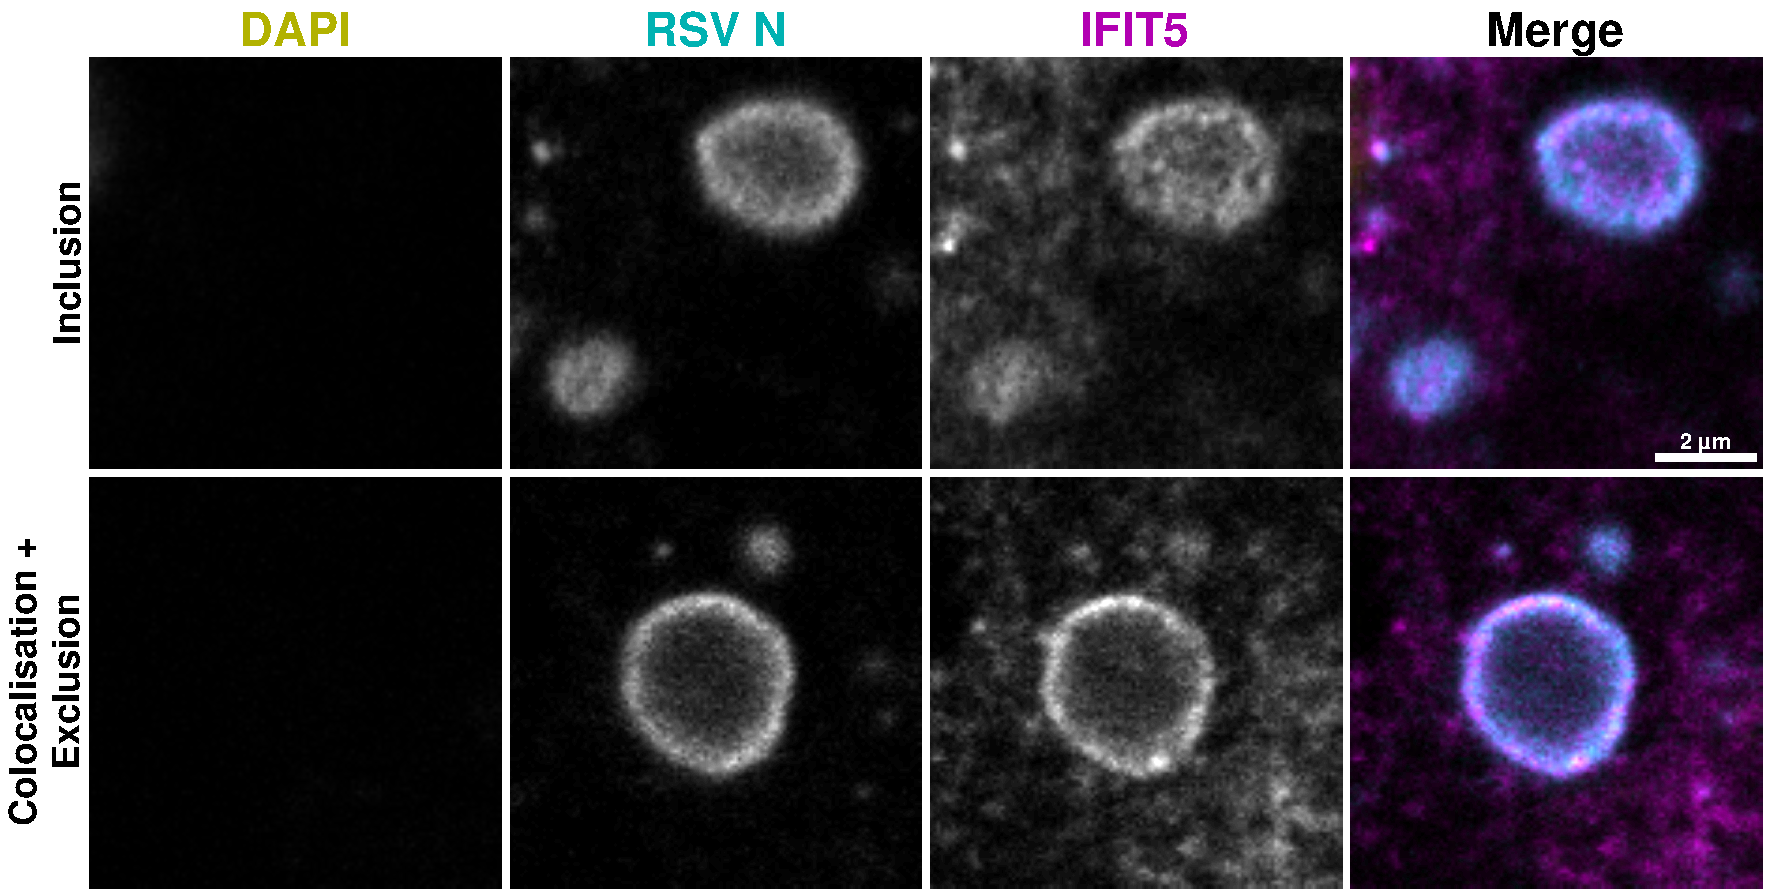
\includegraphics[width=1\linewidth]{09. Chapter 4/Figs/01. pIB/05. IFIT5/03. i5-vero-hnhp.pdf}
    \caption[Representative Images of Interaction Phenotypes of Monkey IFIT5 with Human pIBs in the Vero Cell Line.]{\textbf{Representative Images of Interaction Phenotypes of Monkey IFIT5 with Human pIBs in the Vero Cell Line.} Vero cells were transfected with hRSV N and P containing plasmids using TransIT-X2 and were fixed after 24 hours. Cellular nuclei were stained with DAPI (yellow), and cells were double-labelled with anti-RSV N (cyan) and anti-IFIT5 (magenta) antibodies. This figure showcases representative examples of relevant phenotypes in the interaction between monkey IFIT5 and hRSV pseudo-inclusion bodies. These phenotypes are presented in descending order based on their percentage proportions. The scale bar indicates 2 \(\mu \mbox{m}\).}
    \label{fig:Representative Images of Interaction Phenotypes of Monkey IFIT5 with Human pIBs in the VERO Cell Line}
\end{figure}

Finally, we investigated the interactions of IFIT5 with the simplified model of RSV pseudo-inclusion bodies. As previously mentioned, data was exclusively obtained from the Vero cell line transfected with hRSV \textit{N} and \textit{P}-containing plasmids, allowing us to examine the interaction of monkey IFIT5 with human pIBs. Figure \ref{fig:Interaction Phenotypes of Monkey IFIT5 with Human pIBs in the VERO Cell Line} illustrates the frequencies of occurrences of observed phenotypes, along with the measured pIB areas per observed phenotype, based on 100 recorded observations. Representative images of these phenotypes are shown in Figure \ref{fig:Representative Images of Interaction Phenotypes of Monkey IFIT5 with Human pIBs in the VERO Cell Line}. Monkey IFIT5 displayed two hRSV pIB interaction phenotypes, namely forming intra-pIB inclusions (62\% of observations) and colocalising with the pIB boundary while being excluded from the pIB structure (38\% of observations). The size of inclusion-associated hRSV pIBs ranged from 0.13 \(\mu \mbox{m}^2\) to 10 \(\mu \mbox{m}^2\), with an atypical value of 1.2 \(\mu \mbox{m}^2\). Conversely, the size profile of pIBs associated with colocalisation accompanied by exclusion phenotype ranged from 0.23 \(\mu \mbox{m}^2\) to supra 40, with a median value of 4 \(\mu \mbox{m}^2\). Differentiation of these pIBs based on size is apparent, although there is a marked overlap of sizes where both phenotypes occur (between 0.23 and 10 \(\mu \mbox{m}^2\)). Notably, our previous observations indicated minimal interactions of both human and bovine IFIT5 with RSV inclusion bodies during infection, with the most prevalent observed phenotype being exclusion (Chapter \ref{ch:Subcellular Localisation of Endogenous IFIT Proteins in the Context of RSV Inclusion Bodies}). Specifically, we observed the inclusion phenotype in only 10\% of observations in the MDBK cell line and the colocalisation associated with the exclusion phenotype in 5\% of observations in the A549 cell line. This suggests that IFIT5 has a propensity to interact with pseudo-inclusion bodies, but factors present in RSV IBs during infection may prevent IFIT5 from accessing these structures.

\begin{figure}
    \centering
    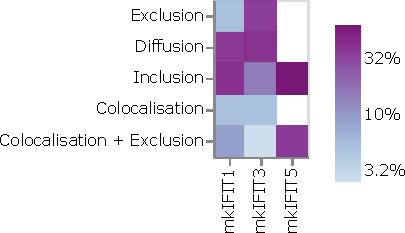
\includegraphics[width=0.6\linewidth]{09. Chapter 4/Figs/heatmap-vero-hnhp-i135.pdf}
    \caption[Summary of the Interactions of Monkey IFIT1, IFIT3, and IFIT5 with hRSV Pseudo Inclusion Bodies.]{\textbf{Summary of the Interactions of Monkey IFIT1, IFIT3, and IFIT5 with hRSV Pseudo Inclusion Bodies.} Heatmap illustrating the frequency of observed interaction phenotypes for monkey IFIT1, IFIT3, and IFIT5 with human pseudo-IBs in Vero cell line. The phenotypes are ordered based on their implication of interaction with the pIBs, with the least interactive on the top and the most interactive on the bottom. The frequencies are presented on a log10 scale to enhance the visualisation of less common phenotypes.}
    \label{fig:Summary of the Interactions of Monkey IFIT1, IFIT3, and IFIT5 with hRSV Pseudo Inclusion Bodies}
\end{figure}

In summary, the investigation of IFIT1, IFIT3, and IFIT5 localisation in the context of the simplified model of RSV inclusion bodies, using ectopically expressed pseudo-inclusion bodies, yielded intriguing results. A summary of these can be seen in Figure \ref{fig:Summary of the Interactions of Monkey IFIT1, IFIT3, and IFIT5 with hRSV Pseudo Inclusion Bodies}. These results provide insights into the nature of their interactions and potential factors impeding these interactions during RSV infection. Concerning endogenous IFIT1, minimal interaction was observed in human cells (HEK293T) with hRSV pIBs, although this may be due to a size bias of the observed pIBs. This assumption is based on observed monkey IFIT1 interactions with human RSV pIBs, where strong interaction phenotypes (inclusion and colocalisation) correlated with increased pIB size. This aligns with results from monkey IFIT1 interaction with bovine RSV pIBs, where only phenotypes implying interaction were observed. Monkey IFIT1 data supports observations from Section \ref{subsec:Endogenous IFIT Interaction with RSV Inclusion Bodies}, where both human and bovine IFIT1 showed strong interaction phenotypes (inclusion or colocalisation) with RSV IBs during infection. However, this was not the dominant observed phenotype, which was exclusion. Monkey IFIT3 exhibited data consistent with what was observed in RSV infection data, i.e., the majority of cases being either indirectly associated with pIBs (diffusion) or excluded from the structures, while directly associating with these structures with small but considerable frequency. This suggests that the IFIT3-IB interaction is directed via biophysical interactions with the pIB and IB structures. Finally, monkey IFIT5 showed only strong interaction phenotypes with human pIBs. This is unexpected, as during infection, neither human nor bovine IFIT5 exhibited minimal direct or indirect interaction phenotypes, with the dominant observed phenotype being exclusion. This discrepancy could be due to the differential propensity of monkey IFIT5 for interaction with (p)IBs compared to human and bovine IFIT5, or it could mean that viral or cellular factors associated with and influencing the RSV IBs during infection prevent IFIT5 from interacting with these structures. While these experiments provided valuable data confirming previous observations (as in the case of IFIT3 or IFIT1 interacting with human pIBs), they also yielded inconsistent results with previous observations. Another issue is that the majority of the gathered data is based on monkey IFITs, which are not relevant for human and bovine RSV infection \textit{in vivo}. Thus, it is essential that this data is further validated and investigated using human and bovine IFITs. To achieve this, we aimed to analyse the interaction profiles of exogenously expressed human and bovine IFITs in the context of human and bovine RSV infection.

\subsection{Overexpressed IFIT1, IFIT3, and IFIT5 During RSV Infection} \label{subsec:Overexpressed IFIT1, IFIT3, and IFIT5 During RSV Infection}
To validate the observed interactions of monkey IFIT1, IFIT3, and IFIT5 with pseudo-inclusion bodies and to explore the maximum potential for interactions between human and bovine IFIT1, IFIT3, and IFIT5 with human and bovine IBs in the context of RSV infection, we conducted IFIT overexpression experiments coupled with RSV infection. Our approach aimed to reduce nonspecific antibody staining by overexpressing FLAG-tagged IFIT proteins, visualised using a monoclonal anti-FLAG antibody. The incorporation of the FLAG tag allowed for enhanced specificity and improved access for IB detection within the phase-separated structures \cite{Munro1984Use70.}. For this purpose, we obtained a library of FLAG-tagged human IFIT1, IFIT2, IFIT3, and IFIT5 ORF-containing plasmids, each tagged with FLAG in the C terminus, from the Viral Gene Expression group at the Pirbright Institute. This group also provided a control GFP-FLAG pcDNA3.1 plasmid, which was used as a control for transfection efficiency and persistence. These were already present in a pcDNA3.1 backbone, which was directly suitable for our downstream analyses. Additionally, we received bovine IFIT-containing plasmids from CVR Glasgow as part of their bovine ISG plasmid library. These plasmids, consisting of SCRPSY backbones optimised for creating lentiviral particles, contained untagged bovine IFIT ORFs. To ensure compatibility with our downstream analyses, we cloned these bovine IFIT ORFs into the pcDNA3.1 plasmid backbone while simultaneously adding a C-terminal FLAG tag.

Detailed schematics and descriptions of the pcDNA3.1 and SCRPSY plasmids are provided in Section \ref{subsec:DNA Plasmids}, and the cloning and subcloning methodologies are elaborated in Sections \ref{subsec:PCR for Cloning into pcDNA3.1} and \ref{subsec:Common Subcloning Methodologies}, respectively. Briefly, forward and reverse primers specific to each bovine IFIT were designed, consisting of, among other elements, sections of the ORF, FLAG tag, start or stop sequences, and recognition sites for Acc65I and NotI restriction enzymes. These were specifically selected as their restriction sites are not present within either of the bovine \textit{IFIT} sequences. These primers facilitated the PCR amplification and isolation of bovine IFIT ORFs from SCRPSY plasmids, which were subsequently subcloned into pcDNA3.1 plasmid backbones.

To investigate the subcellular localisation of exogenously expressed human and bovine IFIT proteins concerning human and bovine RSV inclusion bodies, Vero cells were transfected with 1 \(\mu\)g of \textit{IFIT}-encoding plasmids per well in a 24-well plate using TransIT-X2, as described in Section \ref{subsec:Transfecting Cells}. Subsequently, the cells were infected with MOI 1 RSV following the standard methodology outlined in Section \ref{subsec:Viral Infections, UV-Inactivation and Ruxolitinib Treatment}. Establishing concurrent infection and transfection in the same cells poses inherent challenges. Typically, one treatment induces an antiviral state, hindering further treatment (infection or transfection). To overcome this, various methodologies were explored. Initially, cell transfection was followed by RSV infection 24 hours post-transfection. The GFP-FLAG control plasmid facilitated the assessment of transfection efficiency and persistence, while RSV cytopathic effects (e.g., syncytia formation) confirmed successful infection. Although successful transfection was observed 24 hours post-transfection, no GFP expression was detected after 24 hours of subsequent infection. Subsequently, simultaneous infection and transfection were attempted by first inoculating cells with a virus preparation and incubating for an hour. Following the removal of the inoculum and PBS wash, the transfection mixture was added to the cell culture media. Minimal GFP expression was observed with this approach, despite successful infection. Lastly, initial RSV infection was followed by transfection 24 hours post-infection. Cells were fixed 24 hours post-transfection, i.e., 48 hours post-infection. This methodology yielded the most successful co-infection/transfection, albeit suboptimal, with only 10-15 co-infection/transfection cells detected for some IFIT/RSV combinations. Nevertheless, this quantity sufficed for confocal microscopy analysis.

This outcome is anticipated, given our understanding that overexpressed hIFIT1, hIFIT2, and hIFIT3 exhibit antiviral activity against RSV. Consequently, cells expressing ectopically expressed IFITs create an environment unsuitable for the RSV life cycle. Additionally, as mentioned in Section \ref{subsec:Routes of IFIT Expression Activation}, infected cells activate their innate antiviral pathways, thereby impeding further infection or transfection. This inherent bias results in cells prone to concurrent infection and transfection being non-representative of the general cellular population. Considering the duration of infection, we anticipate a substantial increase in the size of the inclusion bodies after 48 HPI, compared to the observations at 24 HPI. Literature reports indicate that the mean 2D area of bRSV inclusion bodies increased from 8.99 \(\mu \mbox{m}^2\) to 22.18 \(\mu \mbox{m}^2\) between 24 HPI and 48 HPI \cite{Jobe2021BovineResponses}. This complicates the comparison of co-infection/transfection data with the infection data from Chapter \ref{ch:Subcellular Localisation of Endogenous IFIT Proteins in the Context of RSV Inclusion Bodies}. Nevertheless, the present data can be used to explore the potential influence of ectopically expressed IFIT proteins on the 2D IB area, providing insights into their potential anti-RSV mechanisms. Challenges were encountered in obtaining co-infection/transfection data with several plasmids, including bovine IFIT1, human IFIT3, and bovine IFIT5. These difficulties may stem from various factors, such as decreased transfection efficiency due to contaminants in the plasmid preparation or inadequacies in the formation of transfection complexes. All the data presented below are supported by z-stack measurements.

\begin{figure}
    \begin{subfigure}{0.495\textwidth}
        \caption{}
        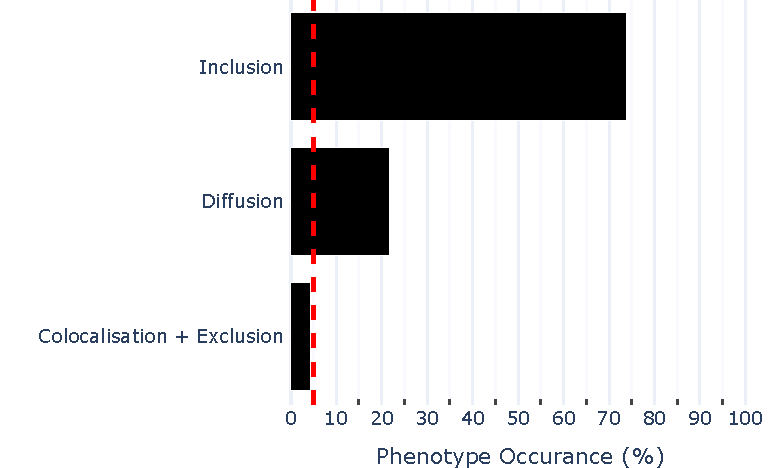
\includegraphics[width=1\linewidth]{09. Chapter 4/Figs/02. Overexpression/01. IFIT1/01. bar_i1_hrsv.pdf} 
    \end{subfigure}
    \begin{subfigure}{0.495\textwidth}
        \caption{}
        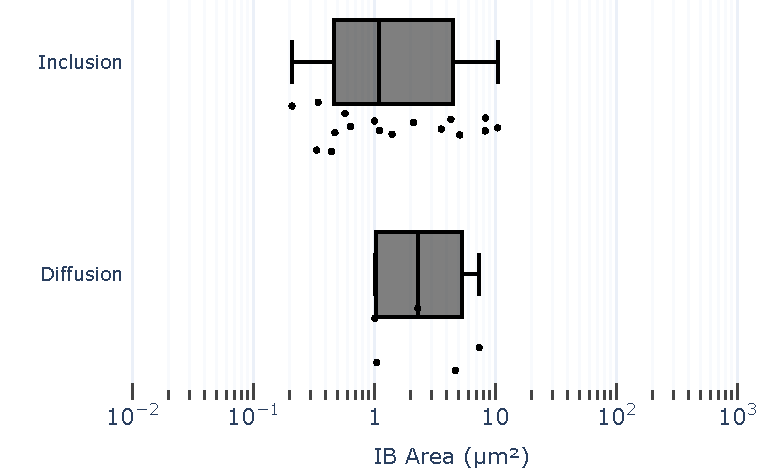
\includegraphics[width=1\linewidth]{09. Chapter 4/Figs/02. Overexpression/01. IFIT1/02. box_i1_hrsv.pdf}
    \end{subfigure}
    \caption[Observed Phenotypes of Exogenous hIFIT1 in the Context of hRSV Inclusion Bodies in Vero Cell Line.]{\textbf{Observed Phenotypes of Exogenous hIFIT1 in the Context of hRSV Inclusion Bodies in Vero Cell Line.} Vero cells were infected with human RSV at MOI 1. 24 HPI, the cells were transfected with hIFIT1-FLAG containing plasmids using TransIT-X2 and were fixed after a further 24 hours. Cells were labelled with anti-RSV N and anti-FLAG antibodies and imaged on a confocal microscope. Panel (a) shows the percentual proportions of observed phenotypes between hRSV inclusion bodies and exogenous hIFIT1 (23 observations), with the red dotted line denoting the 5\% threshold, marking phenotypes considered relevant above this limit. Panel (b) shows the IB area in \(\mu \mbox{m}^2\) per observed relevant phenotype.}
    \label{fig:Observed Phenotypes of Exogenous hIFIT1 in the Context of hRSV Inclusion Bodies in VERO Cell Line}
\end{figure}

\begin{figure}
    \centering
    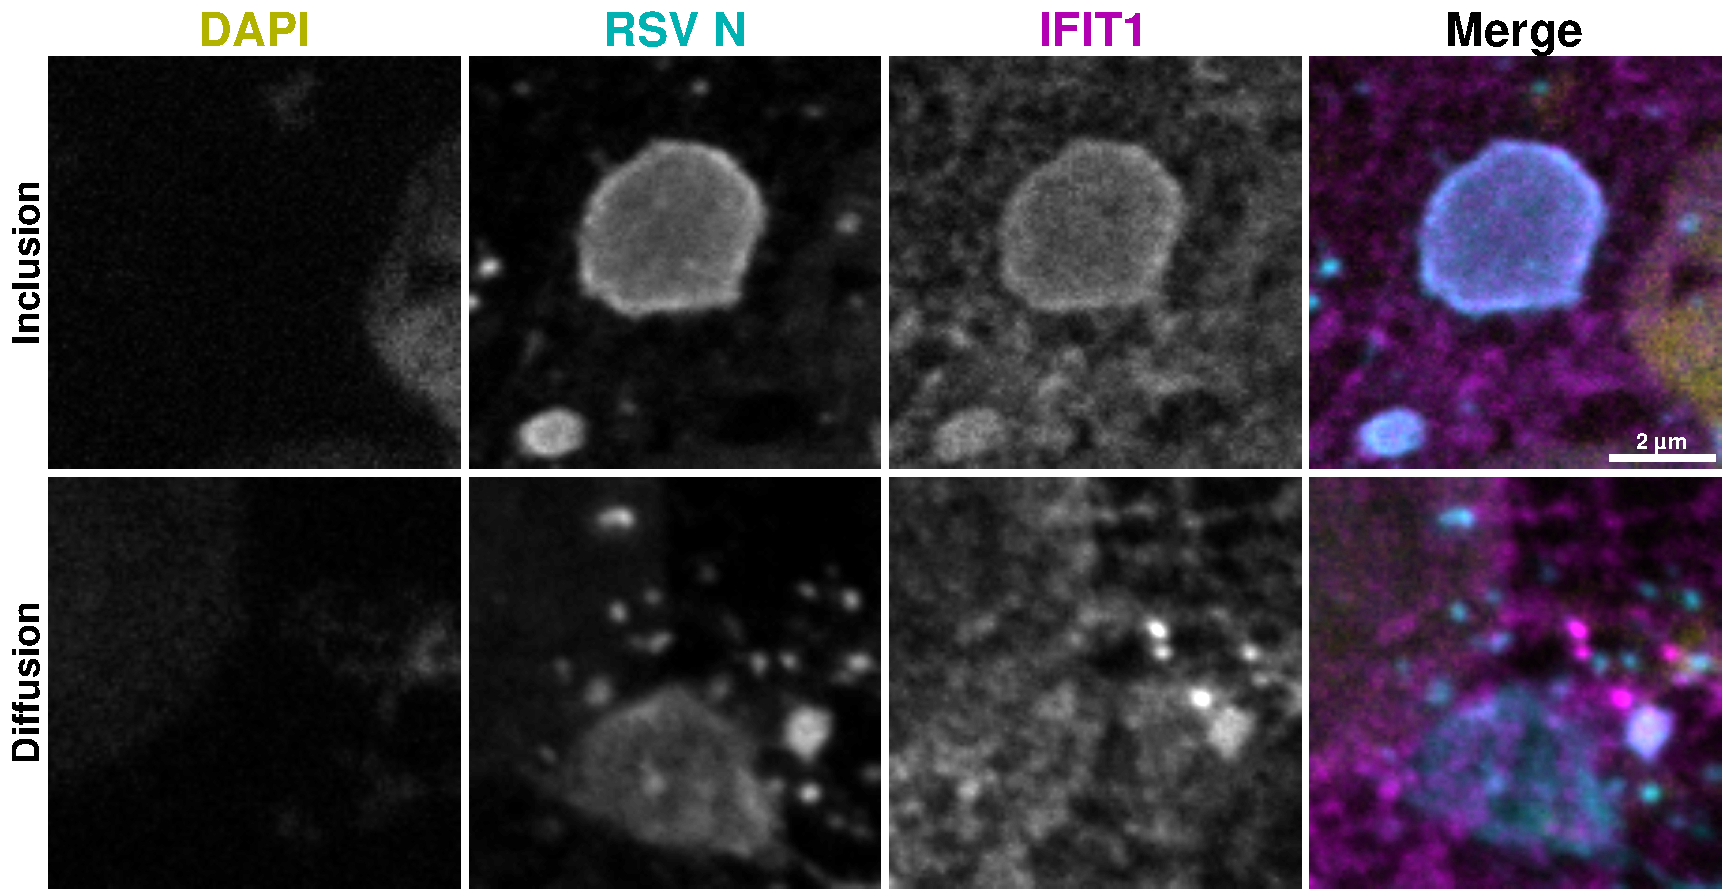
\includegraphics[width=1\linewidth]{09. Chapter 4/Figs/02. Overexpression/01. IFIT1/03. i1-hrsv.pdf}
    \caption[Representative Images of Observed Phenotypes of Exogenous hIFIT1 in the Context of hRSV Inclusion Bodies in Vero Cell Line.]{\textbf{Representative Images of Observed Phenotypes of Exogenous hIFIT1 in the Context of hRSV Inclusion Bodies in Vero Cell Line.} Vero cells were infected with human RSV at MOI 1. 24 HPI, the cells were transfected with hIFIT1-FLAG containing plasmids using TransIT-X2 and were fixed after a further 24 hours. Cellular nuclei were stained with DAPI (yellow), and cells were double-labelled with anti-RSV N (cyan) and anti-FLAG (magenta) antibodies. This figure showcases representative examples of relevant phenotypes in the interaction between exogenous hIFIT1 and hRSV inclusion bodies. These phenotypes are presented in descending order based on their percentage proportions. The scale bar indicates 2 \(\mu \mbox{m}\).}
    \label{fig:Representative Images of Observed Phenotypes of Exogenous hIFIT1 in the Context of hRSV Inclusion Bodies in VERO Cell Line}
\end{figure}

We have documented the expression of human IFIT1 in 23 instances within hRSV-infected cells. The frequencies of observed phenotypes, along with the measured IB sizes of phenotypes occurring with a frequency greater than 5\%, are depicted in Figure \ref{fig:Observed Phenotypes of Exogenous hIFIT1 in the Context of hRSV Inclusion Bodies in VERO Cell Line}. Representative images of these phenotypes are provided in Figure \ref{fig:Representative Images of Observed Phenotypes of Exogenous hIFIT1 in the Context of hRSV Inclusion Bodies in VERO Cell Line}. The most prevalent phenotype was intra-IB inclusion, accounting for 74\% of observations, followed by a diffusion phenotype (22\%), and colocalisation associated with IB exclusion (4\%). The latter, occurring in less than 5\% frequency, was excluded from the size analysis. Concerning the size of IBs associated with the inclusion phenotype, they span the entire size spectrum observed under this condition (i.e., hIFIT1 and hRSV co-infection/transfection), ranging from 0.2 \(\mu \mbox{m}^2\) to 10 \(\mu \mbox{m}^2\), with a typical size of 1.1 \(\mu \mbox{m}^2\). Diffusion-associated IBs were observed to be between 1 \(\mu \mbox{m}^2\) and 7 \(\mu \mbox{m}^2\) in size, with a median value of 2.2 \(\mu \mbox{m}^2\). This indicates that small sub-1 \(\mu \mbox{m}^2\) IBs specifically manifest the inclusion phenotype, while medium-sized IBs display both inclusion and diffusion phenotypes. Interestingly, IBs larger than 10 \(\mu \mbox{m}^2\) were not observed, which is atypical for IBs observed at 48 HPI. This anomaly could be attributed to the anti-RSV action of hIFIT1.

\begin{figure}
    \begin{subfigure}{0.495\textwidth}
        \caption{}
        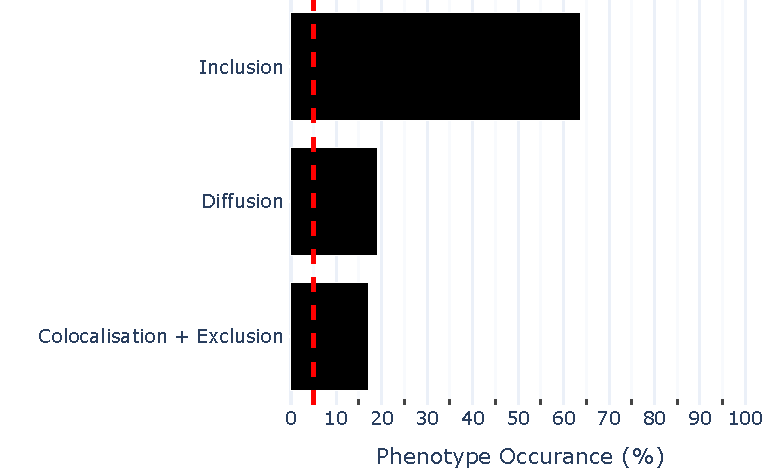
\includegraphics[width=1\linewidth]{09. Chapter 4/Figs/02. Overexpression/01. IFIT1/04. bar_i1_brsv.pdf} 
    \end{subfigure}
    \begin{subfigure}{0.495\textwidth}
        \caption{}
        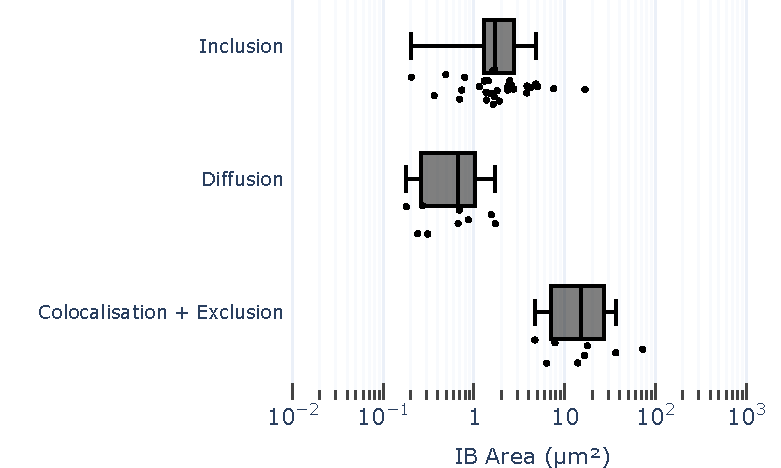
\includegraphics[width=1\linewidth]{09. Chapter 4/Figs/02. Overexpression/01. IFIT1/05. box_i1_brsv.pdf}
    \end{subfigure}
    \caption[Observed Phenotypes of Exogenous hIFIT1 in the Context of bRSV Inclusion Bodies in Vero Cell Line.]{\textbf{Observed Phenotypes of Exogenous hIFIT1 in the Context of bRSV Inclusion Bodies in Vero Cell Line.} Vero cells were infected with bovine RSV at MOI 1. 24 HPI, the cells were transfected with hIFIT1-FLAG containing plasmids using TransIT-X2 and were fixed after a further 24 hours. Cells were labelled with anti-RSV N and anti-FLAG antibodies and imaged on a confocal microscope. Panel (a) shows the percentual proportions of observed phenotypes between bRSV inclusion bodies and exogenous hIFIT1 (47 observations), with the red dotted line denoting the 5\% threshold, marking phenotypes considered relevant above this limit. Panel (b) shows the IB area in \(\mu \mbox{m}^2\) per observed relevant phenotype.}
    \label{fig:Observed Phenotypes of Exogenous hIFIT1 in the Context of bRSV Inclusion Bodies in VERO Cell Line}
\end{figure}

\begin{figure}
    \centering
    \includegraphics[width=1\linewidth]{09. Chapter 4/Figs/02. Overexpression/01. IFIT1/06. i1-brsv.pdf}
    \caption[Representative Images of Observed Phenotypes of Exogenous hIFIT1 in the Context of bRSV Inclusion Bodies in Vero Cell Line.]{\textbf{Representative Images of Observed Phenotypes of Exogenous hIFIT1 in the Context of bRSV Inclusion Bodies in Vero Cell Line.} Vero cells were infected with bovine RSV at MOI 1. 24 HPI, the cells were transfected with hIFIT1-FLAG containing plasmids using TransIT-X2 and were fixed after a further 24 hours. Cellular nuclei were stained with DAPI (yellow), and cells were double-labelled with anti-RSV N (cyan) and anti-FLAG (magenta) antibodies. This figure showcases representative examples of relevant phenotypes in the interaction between exogenous hIFIT1 and bRSV inclusion bodies. These phenotypes are presented in descending order based on their percentage proportions. The scale bar indicates 2 \(\mu \mbox{m}\).}
    \label{fig:Representative Images of Observed Phenotypes of Exogenous hIFIT1 in the Context of bRSV Inclusion Bodies in VERO Cell Line}
\end{figure}

Subsequently, we investigated the interaction of ectopically expressed human IFIT1 with regard to bovine RSV inclusion bodies, resulting in 47 observations. The frequencies of the observed phenotypes, along with the measured IB sizes per associated phenotype, are illustrated in Figure \ref{fig:Observed Phenotypes of Exogenous hIFIT1 in the Context of bRSV Inclusion Bodies in VERO Cell Line}. Representative images are provided in Figure \ref{fig:Representative Images of Observed Phenotypes of Exogenous hIFIT1 in the Context of bRSV Inclusion Bodies in VERO Cell Line}. Similar to the observations during hRSV infection, we identified identical phenotypes with almost identical frequencies. The predominant interaction phenotype was inclusion, occurring in 64\% of observations, followed by the diffusion and colocalisation associated with intra-IB exclusion, observed at 19\% and 16\%, respectively. Notably, we observed a relatively clear differentiation of the phenotypes based on the associated IB areas. While the inclusion-phenotype associated IB areas ranged from 0.2 \(\mu \mbox{m}^2\) to over 10 \(\mu \mbox{m}^2\) with a typical size of 1.8 \(\mu \mbox{m}^2\), most IBs associated with this phenotype clustered between 1 and 5 \(\mu \mbox{m}^2\). The diffusion phenotype occurred in smaller IBs ranging from sub-0.2 \(\mu \mbox{m}^2\) to over 1 \(\mu \mbox{m}^2\), with a median size of 0.8 \(\mu \mbox{m}^2\). Lastly, colocalisation associated with exclusion was exclusively observed in large and very large IBs, ranging from sub-5 \(\mu \mbox{m}^2\) to 70 \(\mu \mbox{m}^2\), with a median size of 14 \(\mu \mbox{m}^2\). Evidently, there is a size separation between IBs associated with either diffusion (small IBs) or colocalisation accompanied by exclusion (large IBs) phenotypes. The inclusion phenotype was most commonly observed in IBs with sizes between these two groups, although it was also observed in extremely sized IBs from both ends. This differentiation could result from the differential maturation status of the inclusion bodies. It is plausible that newly formed small IBs are initially IFIT1-less, although IFIT1 has access to these structures. Subsequently, IFIT1 associates and concentrates inside these structures. As they mature, increase in size and complexity, and become more gel-like, IFIT1 translocates to the periphery of the IB.

\begin{figure}
    \begin{subfigure}{0.495\textwidth}
        \caption{}
        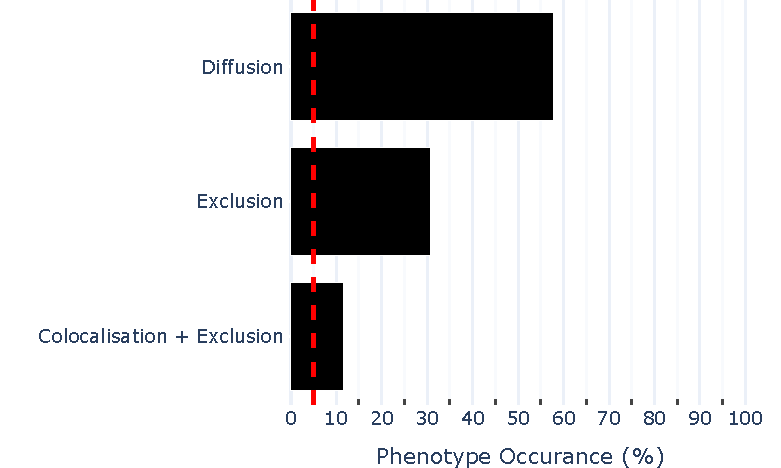
\includegraphics[width=1\linewidth]{09. Chapter 4/Figs/02. Overexpression/03. IFIT3/01. bar_i3_hrsv.pdf} 
    \end{subfigure}
    \begin{subfigure}{0.495\textwidth}
        \caption{}
        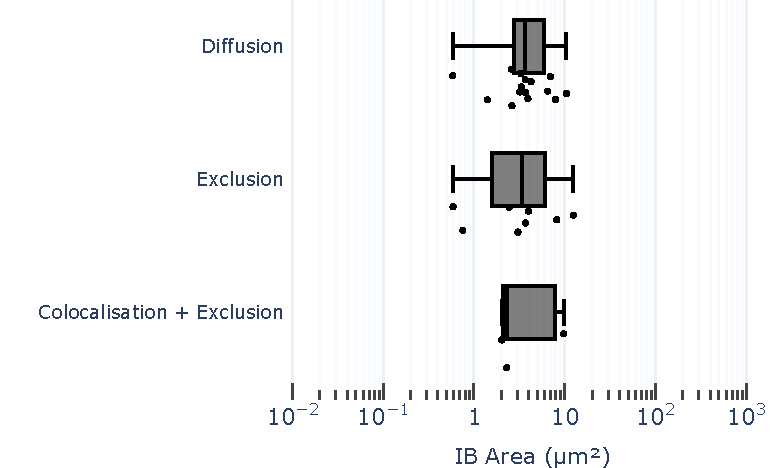
\includegraphics[width=1\linewidth]{09. Chapter 4/Figs/02. Overexpression/03. IFIT3/02. box_i3_hrsv.pdf}
    \end{subfigure}
    \caption[Observed Phenotypes of Exogenous bIFIT3 in the Context of hRSV Inclusion Bodies in Vero Cell Line.]{\textbf{Observed Phenotypes of Exogenous bIFIT3 in the Context of hRSV Inclusion Bodies in Vero Cell Line.} Vero cells were infected with human RSV at MOI 1. 24 HPI, the cells were transfected with bIFIT3-FLAG containing plasmids using TransIT-X2 and were fixed after a further 24 hours. Cells were labelled with anti-RSV N and anti-FLAG antibodies and imaged on a confocal microscope. Panel (a) shows the percentual proportions of observed phenotypes between hRSV inclusion bodies and exogenous bIFIT3 (26 observations), with the red dotted line denoting the 5\% threshold, marking phenotypes considered relevant above this limit. Panel (b) shows the IB area in \(\mu \mbox{m}^2\) per observed relevant phenotype.}
    \label{fig:Observed Phenotypes of Exogenous bIFIT3 in the Context of hRSV Inclusion Bodies in VERO Cell Line}
\end{figure}

\begin{figure}
    \centering
    \includegraphics[width=1\linewidth]{09. Chapter 4/Figs/02. Overexpression/03. IFIT3/03. bi3-hrsv.pdf}
    \caption[Representative Images of Observed Phenotypes of Exogenous bIFIT3 in the Context of hRSV Inclusion Bodies in Vero Cell Line.]{\textbf{Representative Images of Observed Phenotypes of Exogenous bIFIT3 in the Context of hRSV Inclusion Bodies in Vero Cell Line.} Vero cells were infected with human RSV at MOI 1. 24 HPI, the cells were transfected with bIFIT3-FLAG containing plasmids using TransIT-X2 and were fixed after a further 24 hours. Cellular nuclei were stained with DAPI (yellow), and cells were double-labelled with anti-RSV N (cyan) and anti-FLAG (magenta) antibodies. This figure showcases representative examples of relevant phenotypes in the interaction between exogenous bIFIT3 and hRSV inclusion bodies. These phenotypes are presented in descending order based on their percentage proportions. The scale bar indicates 2 \(\mu \mbox{m}\).}
    \label{fig:Representative Images of Observed Phenotypes of Exogenous bIFIT3 in the Context of hRSV Inclusion Bodies in VERO Cell Line}
\end{figure}

Our investigation into the exogenous bovine IFIT3 interaction with hRSV inclusion bodies (IBs) revealed 26 total observations, identifying three interaction phenotypes, each occurring above a 5\% frequency threshold. Figure \ref{fig:Observed Phenotypes of Exogenous bIFIT3 in the Context of hRSV Inclusion Bodies in VERO Cell Line} illustrates the respective phenotypes, their frequencies, and the measured 2D area of the IBs. Representative images of these phenotypes are shown in Figure \ref{fig:Representative Images of Observed Phenotypes of Exogenous bIFIT3 in the Context of hRSV Inclusion Bodies in VERO Cell Line}. Unlike observations with human IFIT1, the predominant phenotypes do not imply interaction. The most commonly observed phenotype was diffusion (57\%), followed by exclusion (31\%), and colocalisation associated with intra-IB exclusion (12\%). Despite slight differences in the median observed IB sizes, all phenotypes were associated with almost identical-sized IBs. Specifically, diffusion-associated IBs ranged in size from 0.6 \(\mu \mbox{m}^2\) to over 10 \(\mu \mbox{m}^2\), with a median value of 4 \(\mu \mbox{m}^2\). Exclusion-associated IBs also ranged in size from 0.6 \(\mu \mbox{m}^2\) to over 10 \(\mu \mbox{m}^2\), with a typical value of 3.3 \(\mu \mbox{m}^2\). Lastly, colocalisation associated with exclusion was observed in three IBs, with sizes of 2 \(\mu \mbox{m}^2\), 2.1 \(\mu \mbox{m}^2\), and 10 \(\mu \mbox{m}^2\). This data suggests that these phenotypes occur independently of IB maturity. Notably, we failed to observe IBs with 2D areas above 10 \(\mu \mbox{m}^2\). This limitation could be attributed to the relatively small number of observations. Alternatively, it may be explained by the seemingly IB-interaction-independent anti-RSV action of bovine IFIT3, restricting the maximum size these structures can attain.

\begin{figure}
    \begin{subfigure}{0.495\textwidth}
        \caption{}
        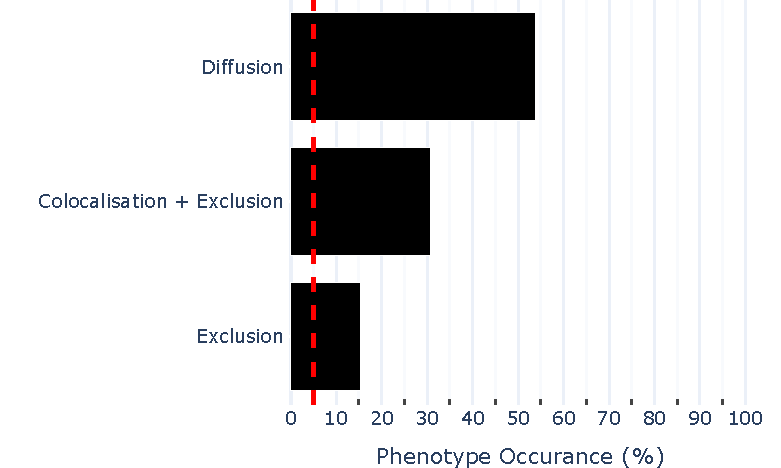
\includegraphics[width=1\linewidth]{09. Chapter 4/Figs/02. Overexpression/03. IFIT3/04. bar_i3_brsv.pdf} 
    \end{subfigure}
    \begin{subfigure}{0.495\textwidth}
        \caption{}
        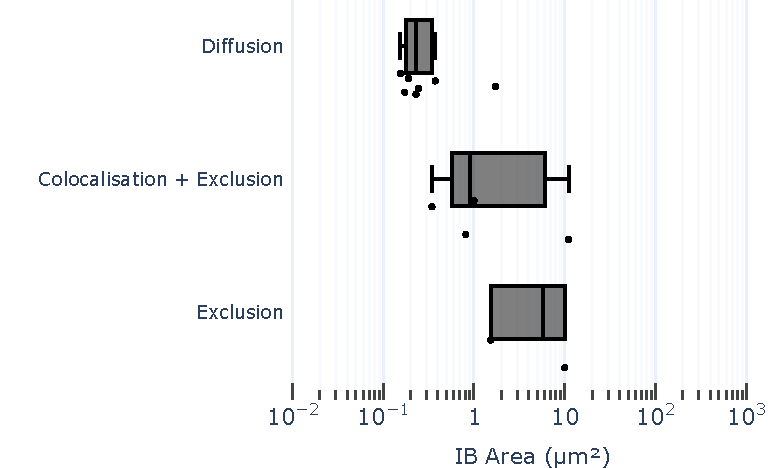
\includegraphics[width=1\linewidth]{09. Chapter 4/Figs/02. Overexpression/03. IFIT3/05. box_i3_brsv.pdf}
    \end{subfigure}
    \caption[Observed Phenotypes of Exogenous bIFIT3 in the Context of bRSV Inclusion Bodies in Vero Cell Line.]{\textbf{Observed Phenotypes of Exogenous bIFIT3 in the Context of bRSV Inclusion Bodies in Vero Cell Line.} Vero cells were infected with bovine RSV at MOI 1. 24 HPI, the cells were transfected with bIFIT3-FLAG containing plasmids using TransIT-X2 and were fixed after a further 24 hours. Cells were labelled with anti-RSV N and anti-FLAG antibodies and imaged on a confocal microscope. Panel (a) shows the percentual proportions of observed phenotypes between bRSV inclusion bodies and exogenous bIFIT3 (13 observations), with the red dotted line denoting the 5\% threshold, marking phenotypes considered relevant above this limit. Panel (b) shows the IB area in \(\mu \mbox{m}^2\) per observed relevant phenotype.}
    \label{fig:Observed Phenotypes of Exogenous bIFIT3 in the Context of bRSV Inclusion Bodies in VERO Cell Line}
\end{figure}

\begin{figure}
    \centering
    \includegraphics[width=1\linewidth]{09. Chapter 4/Figs/02. Overexpression/03. IFIT3/06. bi3-brsv.pdf}
    \caption[Representative Images of Observed Phenotypes of Exogenous bIFIT3 in the Context of bRSV Inclusion Bodies in Vero Cell Line.]{\textbf{Representative Images of Observed Phenotypes of Exogenous bIFIT3 in the Context of bRSV Inclusion Bodies in Vero Cell Line.} Vero cells were infected with bovine RSV at MOI 1. 24 HPI, the cells were transfected with bIFIT3-FLAG containing plasmids using TransIT-X2 and were fixed after a further 24 hours. Cellular nuclei were stained with DAPI (yellow), and cells were double-labelled with anti-RSV N (cyan) and anti-FLAG (magenta) antibodies. This figure showcases representative examples of relevant phenotypes in the interaction between exogenous bIFIT3 and bRSV inclusion bodies. These phenotypes are presented in descending order based on their percentage proportions. The scale bar indicates 2 \(\mu \mbox{m}\).}
    \label{fig:Representative Images of Observed Phenotypes of Exogenous bIFIT3 in the Context of bRSV Inclusion Bodies in VERO Cell Line}
\end{figure}

To validate previous data and ascertain whether the seemingly non-interactive nature of bovine IFIT3 with human IBs is due to species differences, we investigated the interaction phenotypes between ectopically expressed bovine IFIT3 and bovine RSV IBs, resulting in 13 observations. Figure \ref{fig:Observed Phenotypes of Exogenous bIFIT3 in the Context of bRSV Inclusion Bodies in VERO Cell Line} illustrates the observed phenotypes, their frequencies, and the IB sizes. Representative images of these phenotypes are shown in Figure \ref{fig:Representative Images of Observed Phenotypes of Exogenous bIFIT3 in the Context of bRSV Inclusion Bodies in VERO Cell Line}. In 54\% of observations, bovine IFIT3 was observed to be diffused throughout the bRSV IBs. This was followed by colocalisation accompanied by exclusion (31\%) and exclusion (15\%) phenotypes. In contrast to the investigation of exogenous bovine IFIT3 with hRSV IBs, there appears to be a size distinction of IBs associated with different phenotypes. The diffusion phenotype was predominantly observed in very small IBs, ranging from sub-0.2 \(\mu \mbox{m}^2\) to sub-2 \(\mu \mbox{m}^2\), with a median value of 0.9 \(\mu \mbox{m}^2\) where most IBs clustered. Bovine IFIT3 was observed to colocalise with the IB edge while being excluded from the centre of these structures, with IBs having a median size of 0.9 \(\mu \mbox{m}^2\). Lastly, the exclusion phenotype was associated with two IBs of sizes 1.5 \(\mu \mbox{m}^2\) and 10 \(\mu \mbox{m}^2\). It is noteworthy that the observed IB population is of smaller size, and we failed to observe IBs with an area larger than 10 \(\mu \mbox{m}^2\), which is unusual for 48 HPI RSV infection. This anomaly could be attributed to the overall small number of observations or to the potential IB interaction-independent anti-RSV action of bovine IFIT3.

\begin{figure}
    \begin{subfigure}{0.495\textwidth}
        \caption{}
        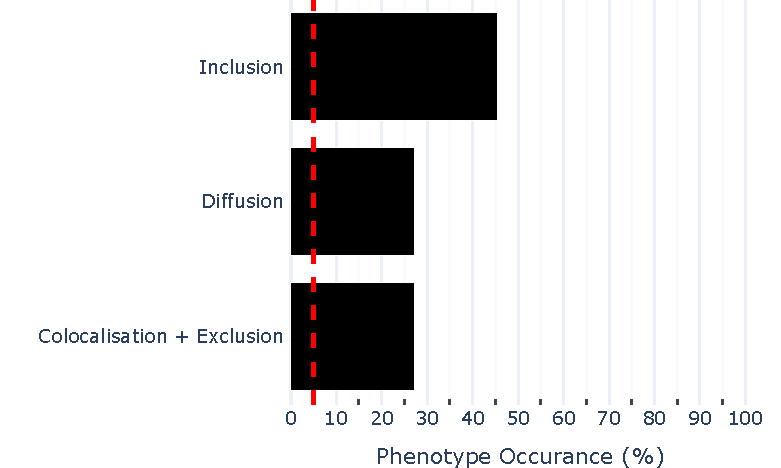
\includegraphics[width=1\linewidth]{09. Chapter 4/Figs/02. Overexpression/04. IFIT5/01. bar_i5_hrsv.pdf} 
    \end{subfigure}
    \begin{subfigure}{0.495\textwidth}
        \caption{}
        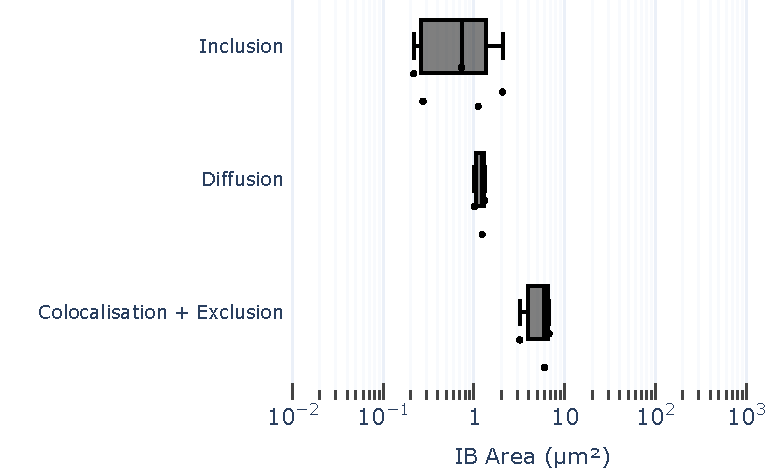
\includegraphics[width=1\linewidth]{09. Chapter 4/Figs/02. Overexpression/04. IFIT5/02. box_i5_hrsv.pdf}
    \end{subfigure}
    \caption[Observed Phenotypes of Exogenous hIFIT5 in the Context of hRSV Inclusion Bodies in Vero Cell Line.]{\textbf{Observed Phenotypes of Exogenous hIFIT5 in the Context of hRSV Inclusion Bodies in Vero Cell Line.} Vero cells were infected with human RSV at MOI 1. 24 HPI, the cells were transfected with hIFIT5-FLAG containing plasmids using TransIT-X2 and were fixed after a further 24 hours. Cells were labelled with anti-RSV N and anti-FLAG antibodies and imaged on a confocal microscope. Panel (a) shows the percentual proportions of observed phenotypes between hRSV inclusion bodies and exogenous hIFIT5 (11 observations), with the red dotted line denoting the 5\% threshold, marking phenotypes considered relevant above this limit. Panel (b) shows the IB area in \(\mu \mbox{m}^2\) per observed relevant phenotype.}
    \label{fig:Observed Phenotypes of Exogenous hIFIT5 in the Context of hRSV Inclusion Bodies in VERO Cell Line}
\end{figure}

\begin{figure}
    \centering
    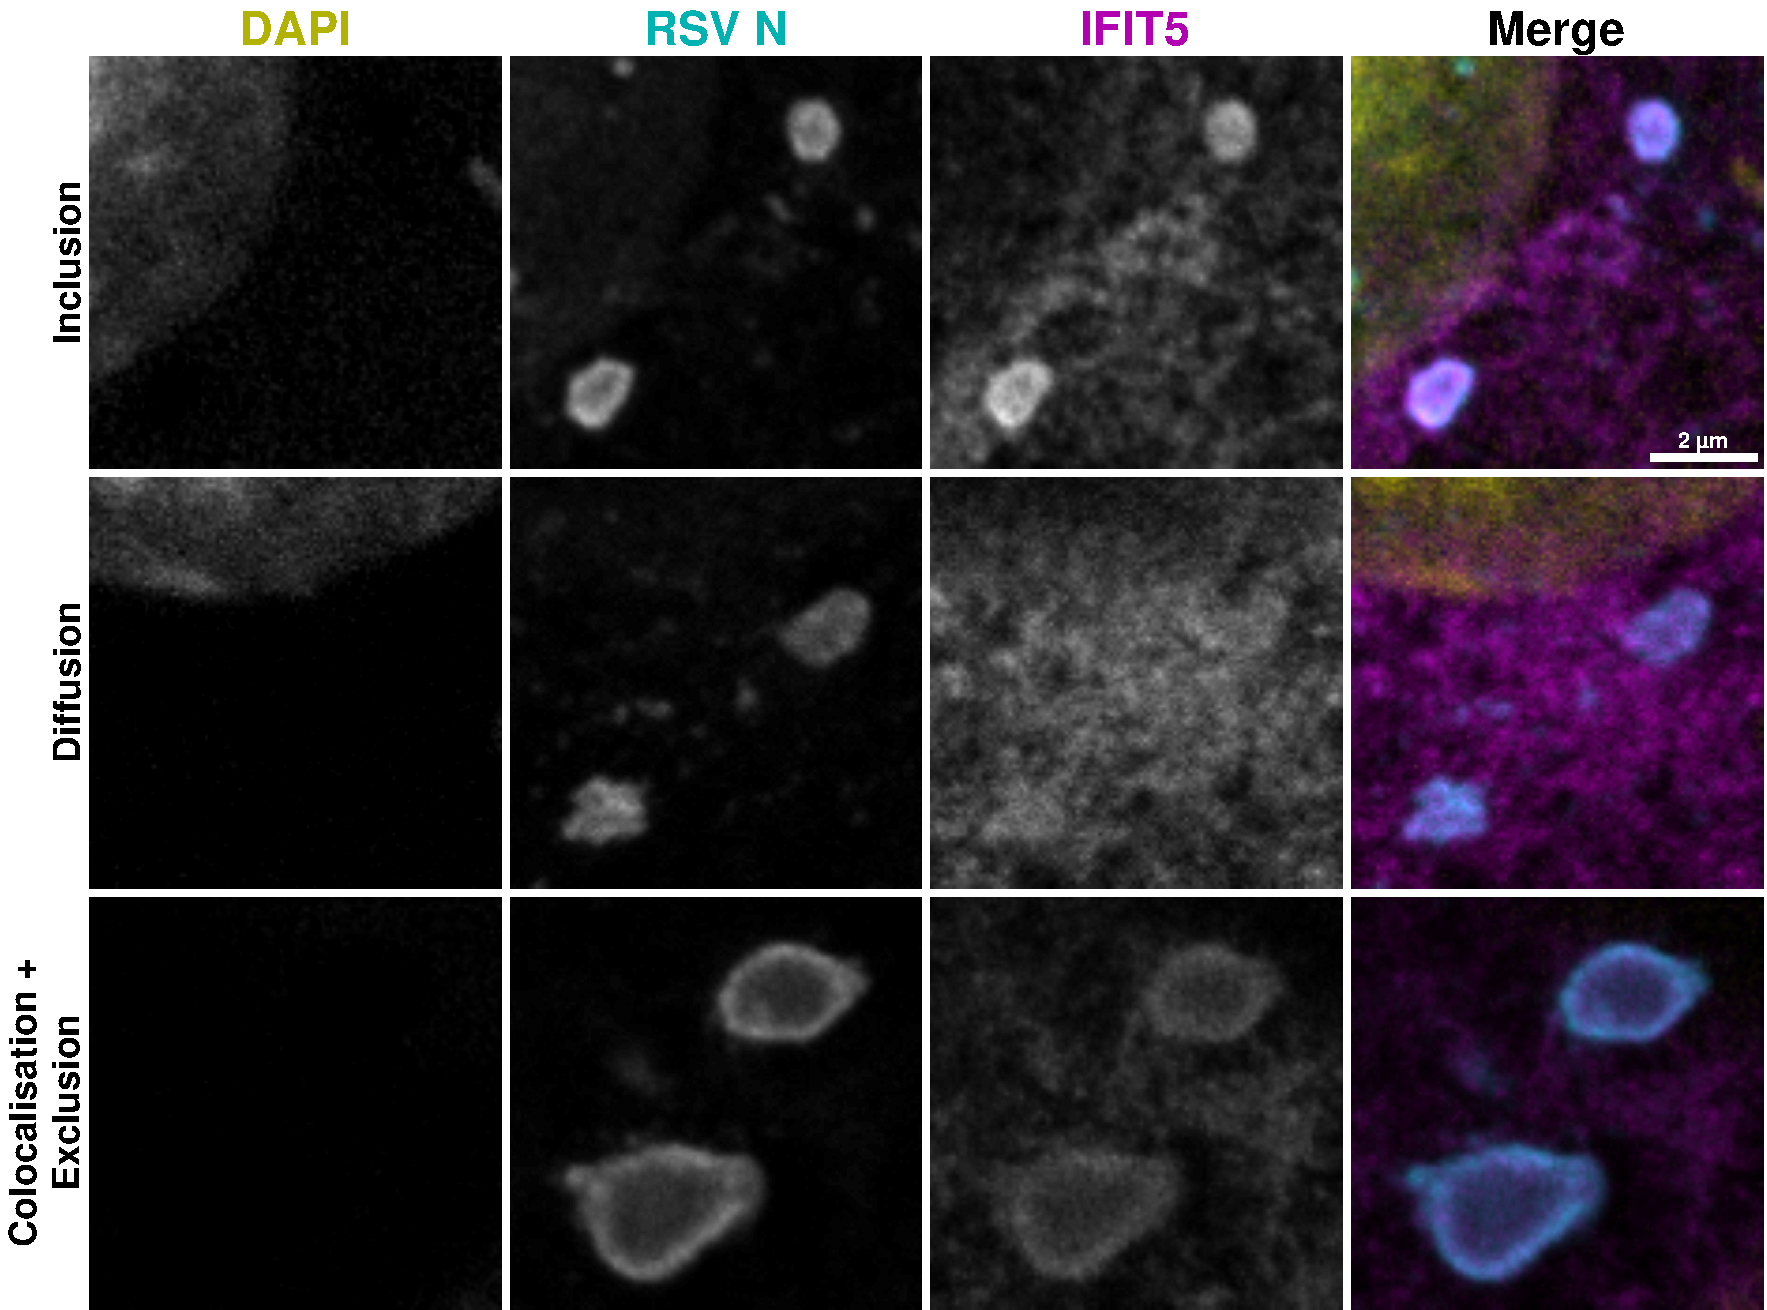
\includegraphics[width=1\linewidth]{09. Chapter 4/Figs/02. Overexpression/04. IFIT5/03. i5-hrsv.pdf}
    \caption[Representative Images of Observed Phenotypes of Exogenous hIFIT5 in the Context of hRSV Inclusion Bodies in Vero Cell Line.]{\textbf{Representative Images of Observed Phenotypes of Exogenous hIFIT5 in the Context of hRSV Inclusion Bodies in Vero Cell Line.} Vero cells were infected with human RSV at MOI 1. 24 HPI, the cells were transfected with hIFIT5-FLAG containing plasmids using TransIT-X2 and were fixed after a further 24 hours. Cellular nuclei were stained with DAPI (yellow), and cells were double-labelled with anti-RSV N (cyan) and anti-FLAG (magenta) antibodies. This figure showcases representative examples of relevant phenotypes in the interaction between exogenous hIFIT5 and hRSV inclusion bodies. These phenotypes are presented in descending order based on their percentage proportions. The scale bar indicates 2 \(\mu \mbox{m}\).}
    \label{fig:Representative Images of Observed Phenotypes of Exogenous hIFIT5 in the Context of hRSV Inclusion Bodies in VERO Cell Line}
\end{figure}

Finally, we investigated the interaction of exogenously expressed human IFIT5 with hRSV inclusion bodies (IBs), resulting in 11 observations and revealing three interaction phenotypes. These phenotypes, along with their associated frequencies of occurrence and the measured IB sizes, are depicted in Figure \ref{fig:Observed Phenotypes of Exogenous hIFIT5 in the Context of hRSV Inclusion Bodies in VERO Cell Line}. Representative images of these phenotypes can be found in Figure \ref{fig:Representative Images of Observed Phenotypes of Exogenous hIFIT5 in the Context of hRSV Inclusion Bodies in VERO Cell Line}. The most commonly observed interaction phenotype was intra-IB inclusion, occurring in 45\% of observations. This was followed by the diffusion and colocalisation associated with exclusion phenotypes, both occurring in 26\% of observations. The inclusion phenotype was associated with relatively small IBs, ranging from sub-0.2 \(\mu \mbox{m}^2\) to 2 \(\mu \mbox{m}^2\) in size, with a median value of 0.7 \(\mu \mbox{m}^2\). Diffusion-associated IBs tightly clustered around their median size of 1.2 \(\mu \mbox{m}^2\). Lastly, the colocalisation associated with exclusion phenotype-associated IBs was larger in size, with a typical size of 6 \(\mu \mbox{m}^2\). It is evident that there is an IB size-dependent distinction of phenotypes. In small, sub-1 \(\mu \mbox{m}^2\) IBs, human IFIT5 concentrates within these structures. As the IBs increase in size and mature, the inclusion phenotype is maintained, but also accompanied by the diffusion phenotype. Lastly, as the IBs further increase in size and reach the limit where IBAGs (inclusion body-associated granules) were reported to form according to the literature, human IFIT5 translocates from the IB interior to the IB boundary. Notably, we have not observed IBs above 7 \(\mu \mbox{m}^2\) in size, suggesting yet again that we are dealing with an incomplete dataset or that the increased concentration of IFIT5 prevents larger IBs from forming.

\begin{figure}
    \begin{subfigure}{0.495\textwidth}
        \caption{}
        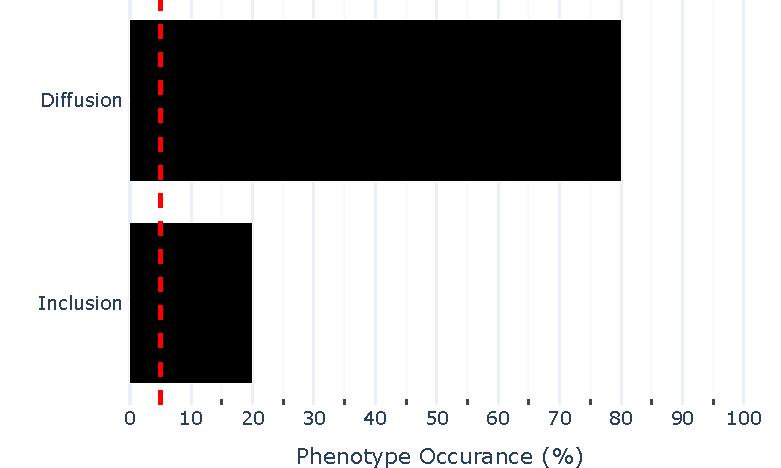
\includegraphics[width=1\linewidth]{09. Chapter 4/Figs/02. Overexpression/04. IFIT5/04. bar_i5_brsv.pdf} 
    \end{subfigure}
    \begin{subfigure}{0.495\textwidth}
        \caption{}
        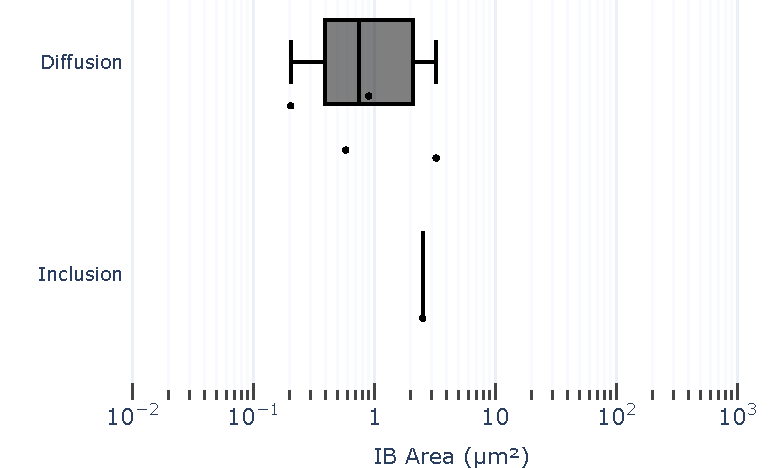
\includegraphics[width=1\linewidth]{09. Chapter 4/Figs/02. Overexpression/04. IFIT5/05. box_i5_brsv.pdf}
    \end{subfigure}
    \caption[Observed Phenotypes of Exogenous hIFIT5 in the Context of bRSV Inclusion Bodies in Vero Cell Line.]{\textbf{Observed Phenotypes of Exogenous hIFIT5 in the Context of bRSV Inclusion Bodies in Vero Cell Line.} Vero cells were infected with bovine RSV at MOI 1. 24 HPI, the cells were transfected with hIFIT5-FLAG containing plasmids using TransIT-X2 and were fixed after a further 24 hours. Cells were labelled with anti-RSV N and anti-FLAG antibodies and imaged on a confocal microscope. Panel (a) shows the percentual proportions of observed phenotypes between bRSV inclusion bodies and exogenous hIFIT5 (5 observations), with the red dotted line denoting the 5\% threshold, marking phenotypes considered relevant above this limit. Panel (b) shows the IB area in \(\mu \mbox{m}^2\) per observed relevant phenotype.}
    \label{fig:Observed Phenotypes of Exogenous hIFIT5 in the Context of bRSV Inclusion Bodies in VERO Cell Line}
\end{figure}

\begin{figure}
    \centering
    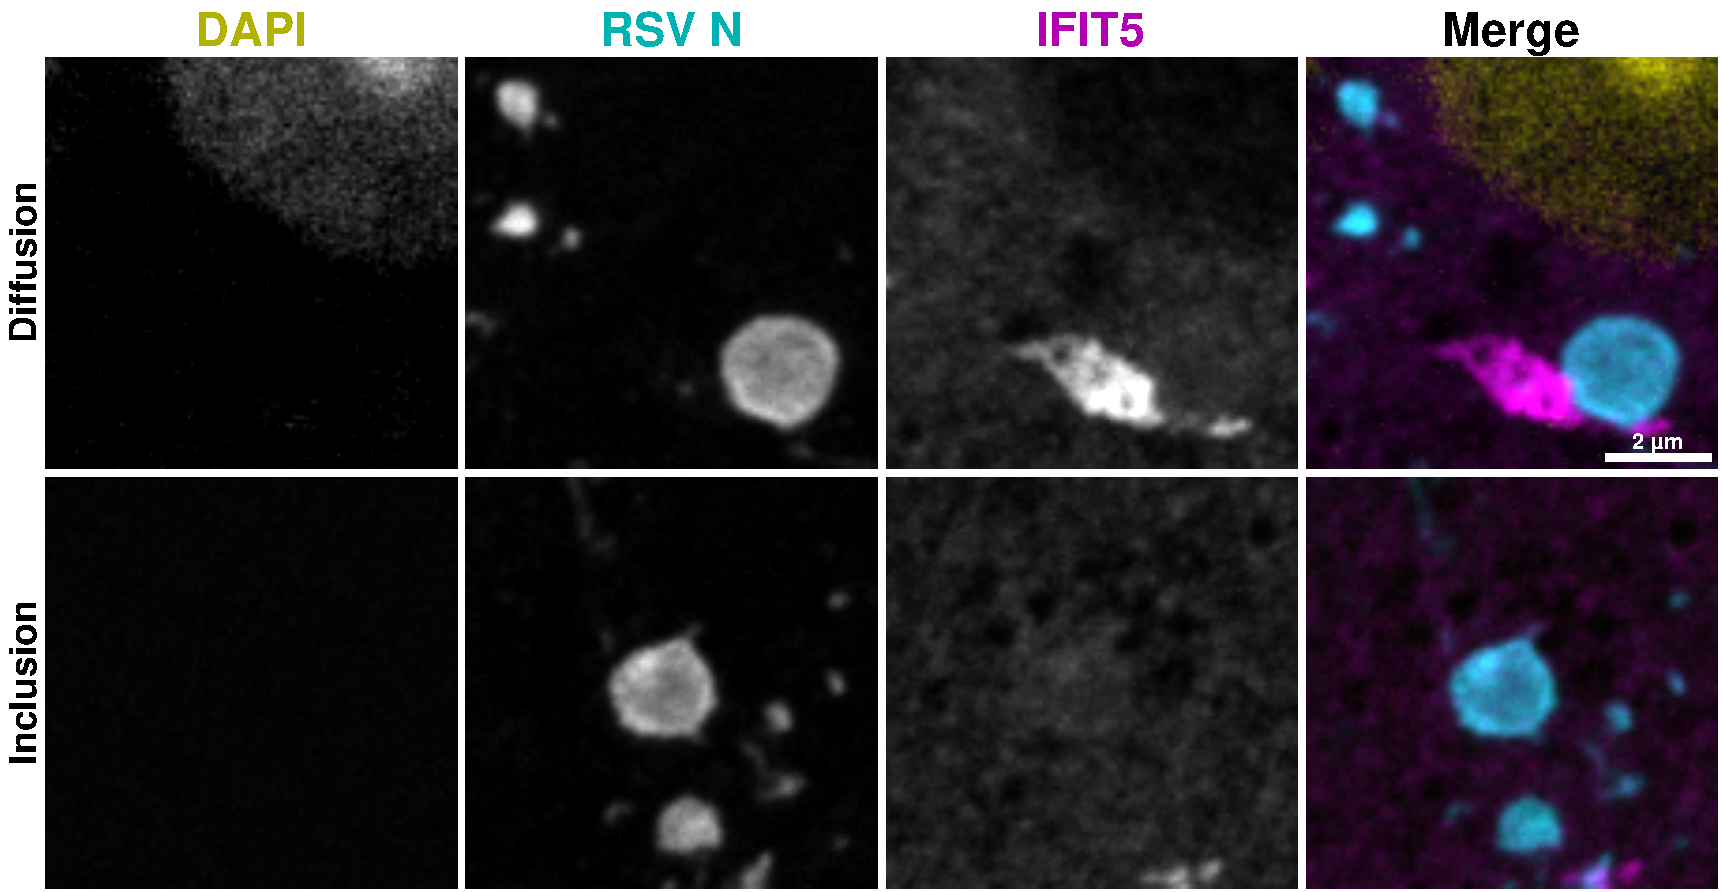
\includegraphics[width=1\linewidth]{09. Chapter 4/Figs/02. Overexpression/04. IFIT5/06. i5-brsv.pdf}
    \caption[Representative Images of Observed Phenotypes of Exogenous hIFIT5 in the Context of bRSV Inclusion Bodies in Vero Cell Line.]{\textbf{Representative Images of Observed Phenotypes of Exogenous hIFIT5 in the Context of bRSV Inclusion Bodies in Vero Cell Line.} Vero cells were infected with bovine RSV at MOI 1. 24 HPI, the cells were transfected with hIFIT5-FLAG containing plasmids using TransIT-X2 and were fixed after a further 24 hours. Cellular nuclei were stained with DAPI (yellow), and cells were double-labelled with anti-RSV N (cyan) and anti-FLAG (magenta) antibodies. This figure showcases representative examples of relevant phenotypes in the interaction between exogenous hIFIT5 and bRSV inclusion bodies. These phenotypes are presented in descending order based on their percentage proportions. The scale bar indicates 2 \(\mu \mbox{m}\).}
    \label{fig:Representative Images of Observed Phenotypes of Exogenous hIFIT5 in the Context of bRSV Inclusion Bodies in VERO Cell Line}
\end{figure}

Lastly, we explored the interaction between exogenously expressed human IFIT5 and bovine RSV IBs, resulting in only 5 observed IB/IFIT5 interactions. Nevertheless, the observed phenotypes, their frequency of occurrence, along with the measured IB areas, are presented in Figure \ref{fig:Observed Phenotypes of Exogenous hIFIT5 in the Context of bRSV Inclusion Bodies in VERO Cell Line}. Representative images of these phenotypes can be found in Figure \ref{fig:Representative Images of Observed Phenotypes of Exogenous hIFIT5 in the Context of bRSV Inclusion Bodies in VERO Cell Line}. The most commonly occurring phenotypic interaction was diffusion, observed in 80\% of observations. IBs associated with this phenotype ranged from 0.2 \(\mu \mbox{m}^2\) to over 3 \(\mu \mbox{m}^2\) in size, with a median measured area of 0.7 \(\mu \mbox{m}^2\). Subsequently, we observed one IB of 2.3 \(\mu \mbox{m}^2\) in size, within which hIFIT5 was concentrated, forming intra-IB inclusion. There seems to be a hint of phenotype separation based on IB size, similar to what we observed previously with hRSV infection (Figure \ref{fig:Observed Phenotypes of Exogenous hIFIT5 in the Context of hRSV Inclusion Bodies in VERO Cell Line}); however, this is challenging to fully assess with only 5 observations. Along these lines, we failed to observe IBs larger than 4 \(\mu \mbox{m}^2\). Based on the hRSV results, we hypothesise that these IBs would exhibit the colocalisation associated with the exclusion phenotype.

Overall, we observed that overexpressed human IFIT1 predominantly formed intra-IB inclusions, exhibited diffusion equally between the cytoplasm and IBs, and colocalised with the edges of large IBs while being excluded from their interior. This pattern remained consistent between hRSV and bRSV infections. However, in bRSV infection, we detected larger IB sizes, resulting in a higher occurrence of the colocalisation associated with the exclusion phenotype. Overexpressed bovine IFIT3 was primarily observed to diffuse throughout hRSV and bRSV IBs, with occasional exclusion or association with IB edges, leading to exclusion from the IB interior. Striking differences in IB sizes associated with these phenotypes were observed between hRSV and bRSV-infected samples. While no difference in sizes was noted for hRSV IBs regarding interaction phenotype association, a clear differentiation of bIFIT3-bRSV IB interaction phenotypes based on IB sizes was evident. The diffusion phenotype predominantly appeared in small, immature IBs, whereas colocalisation was associated with exclusion and the exclusion phenotype occurred in progressively larger IBs. Exogenously expressed human IFIT5 exhibited strong interaction phenotypes with hRSV IBs, namely inclusion and colocalisation associated with exclusion phenotypes, with occasional instances of the diffusion phenotype. Regarding the interaction of overexpressed hIFIT5 with bRSV IBs, the limited observations suggested prevalent diffusion with occasional inclusion. It is possible that gathering a larger dataset, encompassing a broader range of IB sizes, may replicate the results obtained with hRSV. Notably, we failed to observe large IBs (i.e., more than 10 \(\mu \mbox{m}^2\)) in all conditions except for exogenously expressed human IFIT1 during bRSV infection. This observation is unusual, as one would expect inclusion bodies to be more prevalent and larger at the 48 HPI timepoint. This discrepancy may be attributed to the limited number of observations, and repeating the experiments with an increased sample size could unveil more significant IBs. Conversely, the high expression of these IFITs might exert antiviral activity against RSV, potentially preventing the formation of larger IBs.